
\chapter{Stability of defection, optimisation of strategies and the limits of
       memory in the Prisoner's Dilemma.}\label{chapter:memory_one}

\begin{center}
    The research reported in this Chapter has lead to a manuscript, entitled: \\
    \textbf{``A theory of mind: Best responses to memory-one strategies.
    The limitations of extortion and restricted memory''} \\
    Available at: \url{arxiv.org/abs/1911.12112} \\
    Associated data set: \cite{glynatsi2019} \\
    Associated codebase: \cite{Glynatsi2019_opt_mo} \\
    Axelrod-Python library (APL) version: 4.4.0 \\ \vspace{.5cm}
    The manuscript's abstract is the following:
\end{center}

Memory-one strategies are a set of Iterated Prisoner's Dilemma strategies that
have been praised for their mathematical tractability and performance against
single opponents. This manuscript investigates a theory of mind: \textit{best
response} memory-one strategies, as a multidimensional optimisation problem. We
add to the literature that has shown that extortionate play is not always
optimal by showing that optimal play is often not extortionate. We also provide
evidence that memory-one strategies suffer from their limited memory in multi
agent interactions and can be out performed by optimised strategies with longer
memory.

\hrulefill

The differences between the Chapter and the manuscript include details on the
bespoke open source package used to carried out the numerical experiments,
details on resultant theory and an additional section on reactive strategies.
These details and the additional section are only reported in this Chapter, and
not in the manuscript. The Chapter also includes details an introduction to the
Bayesian optimisation used to carry out the numerical experiments.

\section{Introduction}\label{section:mem_one_introduction}

This Chapter contributes to the question: what is the optimal behaviour an IPD
strategy should adapt as a response to different environments?
In~\cite{Press2012} the authors stated that ``Only a player with a theory of
mind about his opponent can do better, in which case Iterated Prisoner's Dilemma
is an Ultimatum Game''. The purpose of this Chapter is to investigate the first
part of this sentence, more specifically, to investigate the best response
strategy with a theory of mind in an environment with memory-one opponents, and
to understand the effects of extortion and restricted memory in those
environments. Extortionate behaviour is explored using a linear algebraic
approach presented in~\cite{Knight2019}.

The outcomes of this Chapter reinforce and extend known results which were presented in
Chapter~\ref{chapter:literature_review}. Namely that memory-one strategies must
adaptable to be successful~\cite{Knight2017, Knight2019} and
that longer-memory strategies have a certain form of advantage over short memory
strategies~\cite{Hilbe2017, Pan2015}. The Chapter is structured as follows:

\begin{itemize}
    \item section~\ref{section:utility} describes a closed form algebraic expression for
    the utility of a memory-one strategy to a given group of opponents.
    \item section~\ref{section:best_response_mem_one} produces a compact method
    of identifying the best response memory-one strategy against a given set
    of memory-one opponents.
    \item section~\ref{section:reactive_strategies} explains best response reactive
    strategies and demonstrates the usage of resultant theory in explicitly finding
    a reactive best response.
    \item section~\ref{section:numerical_experiments} describes a series of numerical experiments
    and a well designed framework that allows the
    comparison of an optimal memory-one strategy and a more complex strategy which
    has a larger memory.
    \item section~\ref{section:stability_of_defection} presents a compact method of identifying environments
    for which cooperation cannot occur.
\end{itemize}


\section{Quadratic form utility of the IPD}\label{section:utility}

One specific advantage of memory-one strategies is their mathematical
tractability. They can be represented completely as an element of \(\R^{4}_{[0, 1]}\).
As previously discussed in Chapter~\ref{chapter:literature_review},
if a strategy is concerned with only the outcome of a single turn then there are
four possible `states' the strategy could be in:

\begin{itemize}
    \item Both players cooperated, denoted as \(CC\).
    \item First player cooperated while the second one defected, denoted as \(CD\).
    \item First player defected while the second one cooperated, denoted as \(DC\).
    \item Both players defected, denoted as \(DD\).
\end{itemize}

Therefore, a memory-one strategy can be denoted by the probability vector of
cooperating after each of these states; \(p=(p_1, p_2, p_3, p_4) \in \R_{[0,1]}
^ 4\).

In~\cite{Nowak1989} it was shown that it is not necessary to simulate the play
of a strategy $p$ against a memory-one opponent $q$. Rather this exact behaviour
can be modelled as a stochastic process, and more specifically as a Markov chain
(Figure~\ref{fig:markov_chain}) whose corresponding transition matrix \(M\) is
given by Equation~(\ref{eq:transition_matrix}). The long run steady state probability
vector \(v\), which is the solution to \(v M = v\), can be
combined with the payoff matrices of Equation~(\ref{eq:pd_definition}) to give the expected
payoffs for each player. More specifically, the utility for a memory-one
strategy \(p\) against an opponent \(q\), denoted as \(u_q(p)\), is given by
Equation~(\ref{eq:press_dyson_utility}).

\begin{figure}
    \centering
    \includestandalone[width=.5\textwidth]{src/chapters/05/tex/markov_chain}
    \caption{Markov Chain}
    \label{fig:markov_chain}
\end{figure}

\begin{equation}\label{eq:transition_matrix}
    M = \left[\begin{matrix}p_{1} q_{1} & p_{1} \left(- q_{1} + 1\right) & q_{1} \left(- p_{1} + 1\right) & \left(- p_{1} + 1\right) \left(- q_{1} + 1\right)\\p_{2} q_{3} & p_{2} \left(- q_{3} + 1\right) & q_{3} \left(- p_{2} + 1\right) & \left(- p_{2} + 1\right) \left(- q_{3} + 1\right)\\p_{3} q_{2} & p_{3} \left(- q_{2} + 1\right) & q_{2} \left(- p_{3} + 1\right) & \left(- p_{3} + 1\right) \left(- q_{2} + 1\right)\\p_{4} q_{4} & p_{4} \left(- q_{4} + 1\right) & q_{4} \left(- p_{4} + 1\right) & \left(- p_{4} + 1\right) \left(- q_{4} + 1\right)\end{matrix}\right]
\end{equation}


\begin{equation}\label{eq:press_dyson_utility}
    u_q(p) = v \cdot (R, S, T, P).
\end{equation}

This thesis is the first work to explore the form of \(u_q(p)\). The first
theoretical result of the thesis is given by
Theorem~\ref{theorem:quadratic_form_u} which states that \(u_q(p)\) is given by
a ratio of two quadratic forms~\cite{kepner2011}.

\begin{theorem}\label{theorem:quadratic_form_u}
    The expected utility of a memory-one strategy \(p\in\mathbb{R}_{[0,1]}^4\)
    against a memory-one opponent \(q\in\mathbb{R}_{[0,1]}^4\), denoted
    as \(u_q(p)\), can be written as a ratio of two quadratic forms:

    \begin{equation}\label{eq:optimisation_quadratic}
    u_q(p) = \frac{\frac{1}{2}pQp^T + cp + a}
                {\frac{1}{2}p\bar{Q}p^T + \bar{c}p + \bar{a}},
    \end{equation}
    where \(Q, \bar{Q}\) \(\in \R^{4\times4}\) are square matrices defined by the
    transition probabilities of the opponent \(q_1, q_2, q_3, q_4\) as follows:

    \begin{center}
    \begin{equation}
    \resizebox{0.91\linewidth}{!}{\arraycolsep=2.5pt%
    \boldmath\(
    Q = \left[\begin{matrix}0 & - \left(q_{1} - q_{3}\right) \left(q_{2} - 5 q_{4} - 1\right) & q_{3} \left(q_{1} - q_{2}\right) & - 5 q_{3} \left(q_{1} - q_{4}\right)\\- \left(q_{1} - q_{3}\right) \left(q_{2} - 5 q_{4} - 1\right) & 0 & \left(q_{2} - q_{3}\right) \left(q_{1} - 3 q_{4} - 1\right) & \left(q_{3} - q_{4}\right) \left(5 q_{1} - 3 q_{2} - 2\right)\\q_{3} \left(q_{1} - q_{2}\right) & \left(q_{2} - q_{3}\right) \left(q_{1} - 3 q_{4} - 1\right) & 0 & 3 q_{3} \left(q_{2} - q_{4}\right)\\- 5 q_{3} \left(q_{1} - q_{4}\right) & \left(q_{3} - q_{4}\right) \left(5 q_{1} - 3 q_{2} - 2\right) & 3 q_{3} \left(q_{2} - q_{4}\right) & 0\end{matrix}\right]\)},
    \end{equation}
    \begin{equation}\label{eq:q_bar_matrix}
    \resizebox{0.91\linewidth}{!}{\arraycolsep=2.5pt%
    \boldmath\(
    \bar{Q} =  \left[\begin{matrix}0 & - \left(q_{1} - q_{3}\right) \left(q_{2} - q_{4} - 1\right) & \left(q_{1} - q_{2}\right) \left(q_{3} - q_{4}\right) & \left(q_{1} - q_{4}\right) \left(q_{2} - q_{3} - 1\right)\\- \left(q_{1} - q_{3}\right) \left(q_{2} - q_{4} - 1\right) & 0 & \left(q_{2} - q_{3}\right) \left(q_{1} - q_{4} - 1\right) & \left(q_{1} - q_{2}\right) \left(q_{3} - q_{4}\right)\\\left(q_{1} - q_{2}\right) \left(q_{3} - q_{4}\right) & \left(q_{2} - q_{3}\right) \left(q_{1} - q_{4} - 1\right) & 0 & - \left(q_{2} - q_{4}\right) \left(q_{1} - q_{3} - 1\right)\\\left(q_{1} - q_{4}\right) \left(q_{2} - q_{3} - 1\right) & \left(q_{1} - q_{2}\right) \left(q_{3} - q_{4}\right) & - \left(q_{2} - q_{4}\right) \left(q_{1} - q_{3} - 1\right) & 0\end{matrix}\right]\)}.
    \end{equation}
    \end{center}

    \(c \text{ and } \bar{c}\) \(\in \R^{4 \times 1}\) are similarly defined by:

    \begin{equation}\label{eq:q_matrix_numerator}
    \resizebox{0.70\linewidth}{!}{\arraycolsep=2.5pt%
    \boldmath\(c = \left[\begin{matrix}q_{1} \left(q_{2} - 5 q_{4} - 1\right)\\- \left(q_{3} - 1\right) \left(q_{2} - 5 q_{4} - 1\right)\\- q_{1} q_{2} + q_{2} q_{3} + 3 q_{2} q_{4} + q_{2} - q_{3}\\5 q_{1} q_{4} - 3 q_{2} q_{4} - 5 q_{3} q_{4} + 5 q_{3} - 2 q_{4}\end{matrix}\right]\),}
    \end{equation}
    \begin{equation}\label{eq:q_matrix_denominator}
    \resizebox{0.35\linewidth}{!}{\arraycolsep=2.5pt%
    \boldmath\(\bar{c} = \left[\begin{matrix}q_{1} \left(q_{2} - q_{4} - 1\right)\\- \left(q_{3} - 1\right) \left(q_{2} - q_{4} - 1\right)\\- q_{1} q_{2} + q_{2} q_{3} + q_{2} - q_{3} + q_{4}\\q_{1} q_{4} - q_{2} - q_{3} q_{4} + q_{3} - q_{4} + 1\end{matrix}\right]\),
    }
    \end{equation}
    and the constant terms \(a, \bar{a}\) are defined as \(a = - q_{2} + 5 q_{4} + 1\) and
    \(\bar{a} = - q_{2} + q_{4} + 1\).
\end{theorem}

\begin{proof}

It was discussed that \(u_q(p)\) it is the product of the steady state
vector \(v\) and the PD payoffs,

\[u_q(p) = v \cdot (R, S, T, P).\]

The dot product of \(v \cdot (R, S, T, P)\) gives,

\begingroup
\scriptsize
\begin{equation*}
    \resizebox{0.91\hsize}{!}{
    $u_q(p) = \left(
    \frac
        {\parbox{6in}{$ - p_{1} p_{2} (q_{1} - q_{3}) (P q_{2} - P - T q_{4}) + p_{1} p_{3} (q_{1} - q_{2}) (P q_{3} - S q_{4}) + p_{1} p_{4} (q_{1} - q_{4}) (S q_{2} - S - T q_{3}) + p_{2} p_{3} (q_{2} - q_{3}) (P q_{1} - P - R q_{4}) - $ \\
        $ p_{2} p_{4} (q_{3} - q_{4}) (R q_{2} - R - T q_{1} + T) + p_{3} p_{4} (q_{2} - q_{4}) (R q_{3} - S q_{1} + S) + p_{1} q_{1} (P q_{2} - P - T q_{4}) - p_{2} (q_{3} - 1) (P q_{2} - P - T q_{4}) + $ \\
        $ p_{3} (- P q_{1} q_{2} + P q_{2} q_{3} + P q_{2} - P q_{3} + R q_{2} q_{4} - S q_{2} q_{4} + S q_{4}) + p_{4} (- R q_{2} q_{4} + R q_{4} + S q_{2} q_{4} - S q_{2} - S q_{4} + S ) $ \\
        \hspace*{5cm} $ T q_{1} q_{4} - T q_{3} q_{4} + T q_{3} - T q_{4} - P q_{2} + P + T q_{4}$
        }}
        {\parbox{6in}{$
        p_{1} p_{2} (q_{1} q_{2} - q_{1} q_{4} - q_{1} - q_{2} q_{3} + q_{3} q_{4} + q_{3}) + p_{1} p_{3} (- q_{1} q_{3} + q_{1} q_{4} + q_{2} q_{3} - q_{2} q_{4}) + p_{1} p_{4} (- q_{1} q_{2} + q_{1} q_{3} + q_{1} + q_{2} q_{4} - q_{3} q_{4} - q_{4}) +$ \\
        $ p_{2} p_{3} (- q_{1} q_{2} + q_{1} q_{3} + q_{2} q_{4} + q_{2} - q_{3} q_{4} - q_{3}) + p_{2} p_{4} (- q_{1} q_{3} + q_{1} q_{4} + q_{2} q_{3} - q_{2} q_{4}) + p_{3} p_{4} (q_{1} q_{2} - q_{1} q_{4} - q_{2} q_{3} - q_{2} + q_{3} q_{4} + q_{4}) + $ \\
        $ p_{1} (- q_{1} q_{2} + q_{1} q_{4} + q_{1}) + p_{2} (q_{2} q_{3} - q_{2} - q_{3} q_{4} - q_{3} + q_{4} + 1) + p_{3} (q_{1} q_{2} - q_{2} q_{3} - q_{2} + q_{3} - q_{4}) + p_{4} (- q_{1} q_{4} + q_{2} + q_{3} q_{4} - q_{3} + q_{4} - 1) + $ \\
        \hspace*{7cm} $q_{2} - q_{4} - 1$
    }}
    \right).$}
\end{equation*}
    \endgroup

Consider the numerator of \(u_q(p)\). The cross product terms \(p_ip_j\) are
given by,

\begingroup
\footnotesize
\begin{align*}
- p_{1} p_{2} (q_{1} - q_{3}) (P q_{2} - P - T q_{4}) + p_{1} p_{3} (q_{1} - q_{2}) (P q_{3} - S q_{4}) + p_{1} p_{4} (q_{1} - q_{4}) (S q_{2} - S - T q_{3}) + \\
p_{2} p_{3} (q_{2} - q_{3}) (P q_{1} - P - R q_{4}) - p_{2} p_{4} (q_{3} - q_{4}) (R q_{2} - R - T q_{1} + T) + p_{3} p_{4} (q_{2} - q_{4}) (R q_{3} - S q_{1} + S)
\end{align*}
\endgroup

This can be re written in a matrix format given by
Equation~(\ref{eq:cross_product_coeffs}).

\begin{equation}\label{eq:cross_product_coeffs}
    \resizebox{0.9\linewidth}{!}{\arraycolsep=2.5pt%
    \boldmath\(
    (p_1, p_2, p_3, p_4) \frac{1}{2} \left[\begin{matrix}0 & - \left(q_{1} - q_{3}\right) \left(q_{2} - 5 q_{4} - 1\right) & q_{3} \left(q_{1} - q_{2}\right) & - 5 q_{3} \left(q_{1} - q_{4}\right)\\- \left(q_{1} - q_{3}\right) \left(q_{2} - 5 q_{4} - 1\right) & 0 & \left(q_{2} - q_{3}\right) \left(q_{1} - 3 q_{4} - 1\right) & \left(q_{3} - q_{4}\right) \left(5 q_{1} - 3 q_{2} - 2\right)\\q_{3} \left(q_{1} - q_{2}\right) & \left(q_{2} - q_{3}\right) \left(q_{1} - 3 q_{4} - 1\right) & 0 & 3 q_{3} \left(q_{2} - q_{4}\right)\\- 5 q_{3} \left(q_{1} - q_{4}\right) & \left(q_{3} - q_{4}\right) \left(5 q_{1} - 3 q_{2} - 2\right) & 3 q_{3} \left(q_{2} - q_{4}\right) & 0\end{matrix}\right] \begin{pmatrix}
    p_1 \\
    p_2 \\
    p_3 \\
    p_4 \end{pmatrix}
    \) }
\end{equation}

Similarly, the linear terms are given by,

\begingroup
\footnotesize
\begin{align*}
p_{1} q_{1} & (P q_{2} - P - T q_{4}) + p_{4} (- R q_{2} q_{4} + R q_{4} + S q_{2} q_{4} - S q_{2} - S q_{4} + S + T q_{1} q_{4} - T q_{3} q_{4} + T q_{3} - T q_{4})\\
- p_{2} & (q_{3} - 1) (P q_{2} - P - T q_{4}) + p_{3} (- P q_{1} q_{2} + P q_{2} q_{3} + P q_{2} - P q_{3} + R q_{2} q_{4} - S q_{2} q_{4} + S q_{4})
\end{align*}
\endgroup

and the expression can be written using a matrix format as
Equation~(\ref{eq:linear_coeffs}).

\begin{equation}\label{eq:linear_coeffs}
    \resizebox{0.7\linewidth}{!}{\arraycolsep=2.5pt%
    \boldmath\(
    (p_1, p_2, p_3, p_4) \left[\begin{matrix}q_{1} \left(q_{2} - 5 q_{4} - 1\right)\\- \left(q_{3} - 1\right) \left(q_{2} - 5 q_{4} - 1\right)\\- q_{1} q_{2} + q_{2} q_{3} + 3 q_{2} q_{4} + q_{2} - q_{3}\\5 q_{1} q_{4} - 3 q_{2} q_{4} - 5 q_{3} q_{4} + 5 q_{3} - 2 q_{4}\end{matrix}\right]\)}
\end{equation}

Finally, the constant term of the numerator, which is obtained by
substituting $p=(0, 0, 0, 0)$, is given by Equation~(\ref{eq:constant}).

\begin{equation}\label{eq:constant}
- P q_{2} + P + T q_{4}
\end{equation}

Combining Equation~(\ref{eq:cross_product_coeffs}), Equation~(\ref{eq:linear_coeffs}) and
Equation~(\ref{eq:constant}) gives that the numerator of \(u_q(p)\) can be written
as,

\begingroup
\boldmath
\begin{equation*}
\resizebox{0.9\textwidth}{!}{$ \begin{split}
    \frac{1}{2}p & \left[\begin{matrix}0 & - \left(q_{1} - q_{3}\right) \left(q_{2} - 5 q_{4} - 1\right) & q_{3} \left(q_{1} - q_{2}\right) & - 5 q_{3} \left(q_{1} - q_{4}\right)\\- \left(q_{1} - q_{3}\right) \left(q_{2} - 5 q_{4} - 1\right) & 0 & \left(q_{2} - q_{3}\right) \left(q_{1} - 3 q_{4} - 1\right) & \left(q_{3} - q_{4}\right) \left(5 q_{1} - 3 q_{2} - 2\right)\\q_{3} \left(q_{1} - q_{2}\right) & \left(q_{2} - q_{3}\right) \left(q_{1} - 3 q_{4} - 1\right) & 0 & 3 q_{3} \left(q_{2} - q_{4}\right)\\- 5 q_{3} \left(q_{1} - q_{4}\right) & \left(q_{3} - q_{4}\right) \left(5 q_{1} - 3 q_{2} - 2\right) & 3 q_{3} \left(q_{2} - q_{4}\right) & 0\end{matrix}\right] p^T +  \\
    & \left[\begin{matrix}q_{1} \left(q_{2} - 5 q_{4} - 1\right)\\- \left(q_{3} - 1\right) \left(q_{2} - 5 q_{4} - 1\right)\\- q_{1} q_{2} + q_{2} q_{3} + 3 q_{2} q_{4} + q_{2} - q_{3}\\5 q_{1} q_{4} - 3 q_{2} q_{4} - 5 q_{3} q_{4} + 5 q_{3} - 2 q_{4}\end{matrix}\right] p - P q_{2} + P + T q_{4}
\end{split} $}
\end{equation*}
\endgroup

and equivalently as,

\[\frac{1}{2}pQp^T + cp + a\]

where \(Q\) \(\in \R^{4\times4}\) is a square matrix defined by the
transition probabilities of the opponent \(q_1, q_2, q_3, q_4\) as follows:

\begin{equation*}
    \resizebox{0.9\linewidth}{!}{\arraycolsep=2.5pt%
    \boldmath\(
    Q = \left[\begin{matrix}0 & - \left(q_{1} - q_{3}\right) \left(q_{2} - 5 q_{4} - 1\right) & q_{3} \left(q_{1} - q_{2}\right) & - 5 q_{3} \left(q_{1} - q_{4}\right)\\- \left(q_{1} - q_{3}\right) \left(q_{2} - 5 q_{4} - 1\right) & 0 & \left(q_{2} - q_{3}\right) \left(q_{1} - 3 q_{4} - 1\right) & \left(q_{3} - q_{4}\right) \left(5 q_{1} - 3 q_{2} - 2\right)\\q_{3} \left(q_{1} - q_{2}\right) & \left(q_{2} - q_{3}\right) \left(q_{1} - 3 q_{4} - 1\right) & 0 & 3 q_{3} \left(q_{2} - q_{4}\right)\\- 5 q_{3} \left(q_{1} - q_{4}\right) & \left(q_{3} - q_{4}\right) \left(5 q_{1} - 3 q_{2} - 2\right) & 3 q_{3} \left(q_{2} - q_{4}\right) & 0\end{matrix}\right]\)},
\end{equation*}

\(c\) \(\in \R^{4 \times 1}\) is similarly defined by:

\begin{equation*}
    \resizebox{0.6\linewidth}{!}{\arraycolsep=2.5pt%
    \boldmath\(c = \left[\begin{matrix}q_{1} \left(q_{2} - 5 q_{4} - 1\right)\\- \left(q_{3} - 1\right) \left(q_{2} - 5 q_{4} - 1\right)\\- q_{1} q_{2} + q_{2} q_{3} + 3 q_{2} q_{4} + q_{2} - q_{3}\\5 q_{1} q_{4} - 3 q_{2} q_{4} - 5 q_{3} q_{4} + 5 q_{3} - 2 q_{4}\end{matrix}\right]\),}
\end{equation*}

and \(a = - q_{2} + 5 q_{4} + 1\).

The same process is done for the denominator.
\end{proof}

Numerical simulations have been carried out to validate the result. The simulated utility, which is
denoted as \(U_q(p)\), has been calculated with APL.
For smoothing the simulated results the utility
has been estimated in a tournament of 500 turns and 200 repetitions.
Figure~\ref{fig:analytical_simulated} shows two examples demonstrating that the
formulation of Theorem~\ref{theorem:quadratic_form_u} successfully captures the
simulated behaviour.

\begin{figure}[!htbp]
    \begin{center}
        \begin{subfigure}{0.5\textwidth}
            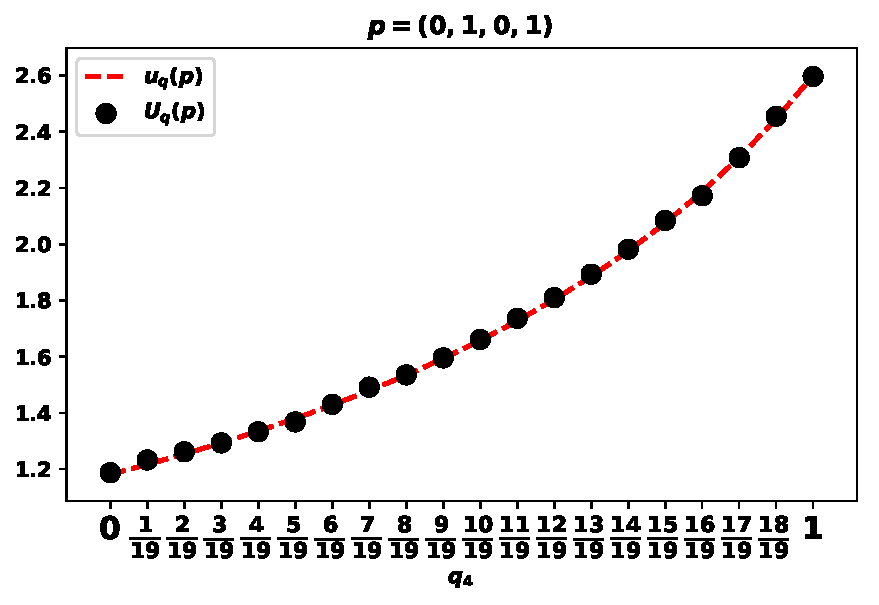
\includegraphics[width=\linewidth]{src/chapters/05/paper/memory-size-in-the-prisoners-dilemma/img/validation_against_player_one.pdf}
        \end{subfigure}
        \begin{subfigure}{0.5\textwidth}
            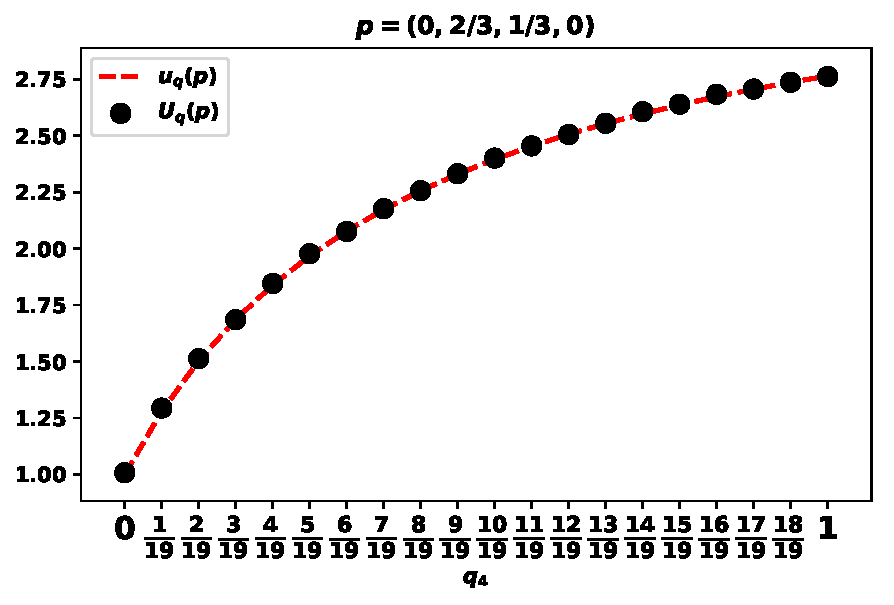
\includegraphics[width=\linewidth]{src/chapters/05/paper/memory-size-in-the-prisoners-dilemma/img/validation_against_player_two.pdf}
        \end{subfigure}
    \end{center}
    \caption{Simulated and empirical utilities for \(p = (0, 1, 0, 1)\)
    and \(p = (0, \frac{2}{3}, \frac{1}{3}, 0)\) against \((\frac{1}{3}, \frac{1}{3}, \frac{1}{3}, q_4)\) for
    \(q_4 \in \{0,  \frac{1}{19}, \frac{2}{19}, \dots, \frac{18}{19}, 1\}\).
    \(u_q(p)\) is the theoretic value given in Theorem~\ref{theorem:quadratic_form_u},
    and \(U_q(p)\) is simulated numerically using APL.}
    \label{fig:analytical_simulated}
\end{figure}

Theorem~\ref{theorem:quadratic_form_u} can be extended to consider multiple
opponents. The IPD is commonly studied in tournaments and/or Moran Processes~\cite{Kaiping2014}
where a strategy interacts with a number of opponents. The payoff of a player in
such interactions is given by the average payoff the player received against
each opponent. More specifically the expected utility of a memory-one strategy
against \(N\) opponents is given by Theorem~\ref{theorem:tournament_utility}.

\begin{theorem}\label{theorem:tournament_utility}
    The expected utility of a memory-one strategy \(p\in\mathbb{R}_{[0,1]}^4\)
    against a group of opponents \(\{q^{(1)}, q^{(2)}, \dots, q^{(N)}\}\), denoted
    as \(\frac{1}{N} \sum\limits_{i=1} ^ {N} {u_q}^{(i)} (p)\), is given by:

    \begin{equation}\label{eq:tournament_utility}
        \frac{1}{N} \sum\limits_{i=1} ^ {N} {u_q}^{(i)} (p) = \frac{1}{N}
        \frac{\sum\limits_{i=1} ^ {N} (\frac{1}{2} pQ^{(i)} p^T + c^{(i)} p + a^ {(i)})
        \prod\limits_{\tiny\begin{array}{l} j=1 \\ j \neq i \end{array}} ^
        N (\frac{1}{2} p\bar{Q}^{(j)} p^T + \bar{c}^{(j)} p + \bar{a}^ {(j)})}
        {\prod\limits_{i=1} ^ N (\frac{1}{2} p\bar{Q}^{(i)} p^T + \bar{c}^{(i)} p + \bar{a}^ {(i)})}.
    \end{equation}
\end{theorem}

Equation~(\ref{eq:tournament_utility}) is the average score
(using Equation~(\ref{eq:optimisation_quadratic})) against the set of opponents.

Similar to the previous result, the formulation of
Theorem~\ref{theorem:tournament_utility} is validated using numerical
simulations where the 10 memory-one strategies described in~\cite{Stewart2012}
have been used as the opponents. Figure~\ref{fig:stewart_plotkin_results} shows
that the simulated behaviour has been captured successfully.

\begin{figure}[!htbp]
    \begin{center}
    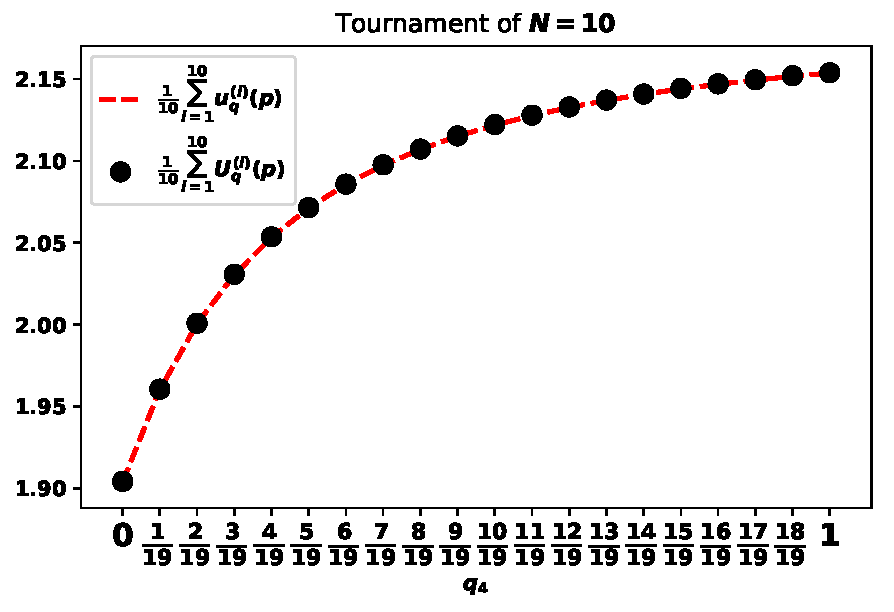
\includegraphics[width=.5\linewidth]{src/chapters/05/paper/memory-size-in-the-prisoners-dilemma/img/Stewart_tournament_results.pdf}
    \caption{The utilities of memory-one strategies \((\frac{1}{3}, \frac{1}{3}, \frac{1}{3}, p_4)\) for
    \(p_4 \in \{0,  \frac{1}{19}, \frac{2}{19}, \dots, \frac{18}{19}, 1\}\)
    against the 10 memory-one strategies described in~\cite{Stewart2012}.
    \(\frac{1}{10} \sum^{10}_{i=1} u_q^{(i)}(p)\) is the theoretic value given in
    Theorem~\ref{theorem:quadratic_form_u},
    and \(\frac{1}{10} \sum^{10}_{i=1} U_q^{(i)}(p)\) is simulated numerically
    using APL.}
    \label{fig:stewart_plotkin_results}
    \end{center}
\end{figure}

The list of strategies from~\cite{Stewart2012} was also used to check whether
the utility against a group of strategies could be captured by the utility
against the mean opponent. Thus whether condition (\ref{eq:condition}) holds.
However condition~(\ref{eq:condition}) fails, as shown in
Figure~\ref{fig:hypothesis}.

\begin{equation}\label{eq:condition}
    \frac{1}{N} \sum_{i=1} ^ {N} {u_q}^{(i)} (p) = u_{\frac {1}{N} \sum\limits_{i=1} ^ N q^{(i)}}(p),
\end{equation}

\begin{figure}[!htbp]
    \begin{center}
    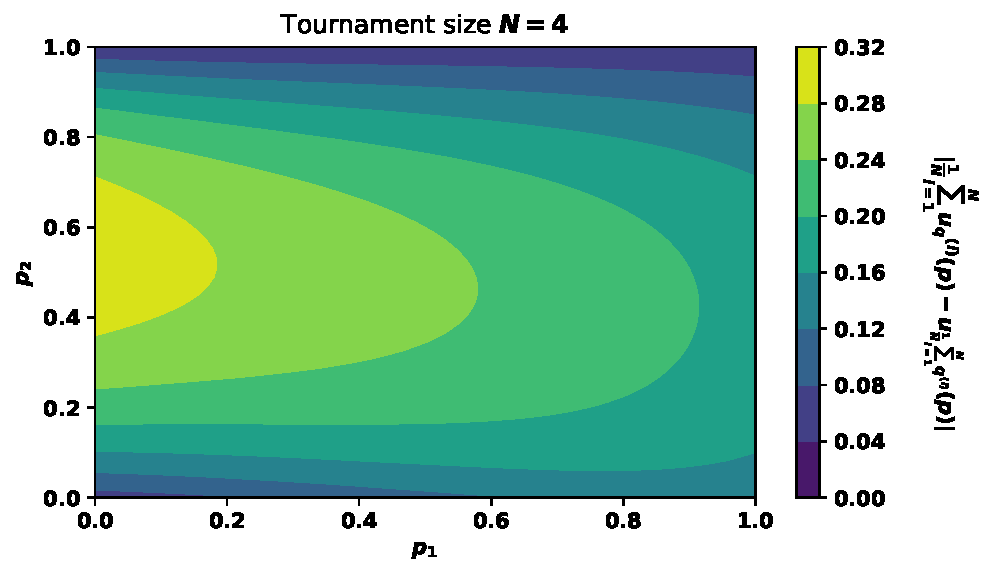
\includegraphics[width=.6\linewidth]{src/chapters/05/paper/memory-size-in-the-prisoners-dilemma/img/mean_vs_average_heatmap.pdf}
    \end{center}
    \caption{The difference between the average utility against the opponents
    from~\cite{Stewart2012} and the utility against the average player of the
    strategies in~\cite{Stewart2012} of a player \(p=(p_1, p_2, p_1, p_2)\). A
    positive difference indicates that condition (\ref{eq:condition}) does not
    hold.}
    \label{fig:hypothesis}
\end{figure}

Theorem~\ref{theorem:tournament_utility} which allows for the utility of a
memory-one strategy against any number of opponents to be estimated without
simulating the interactions is the main result used in the rest of this Chapter. In
section~\ref{section:best_response_mem_one} it is used to define best response
memory-one strategies, in section~\ref{section:reactive_strategies} to define best response
reactive strategies and in section~\ref{section:stability_of_defection}
to explore the conditions under which defection dominates cooperation.

\section{Best responses to memory-one players}\label{section:best_response_mem_one}

This section focuses on \textit{memory-one
best response} strategies. A best response is a strategy which
corresponds to the most favourable outcome (Chapter~\ref{chapter:introduction}), thus a memory-one
best response to a set of opponents \(q^{(1)}, q^{(2)}, \dots, q^{(N)}\) corresponds to a strategy \(p^*\) for which
Equation (\ref{eq:tournament_utility}) is maximised. This is considered as a multi
dimensional optimisation problem given by:

\begin{equation}\label{eq:mo_tournament_optimisation}
    \begin{aligned}
    \max_p: & \ \sum_{i=1} ^ {N} {u_q}^{(i)} (p)
    \\
    \text{such that}: & \ p \in \R_{[0, 1]}
    \end{aligned}
\end{equation}

Optimising this particular ratio of quadratic forms is not trivial. It can be
verified empirically for the case of a single opponent that there exists at
least one point for which the definition of concavity does not hold.

A function \(f(x)\) is concave on an interval \([a, b]\) if, for any two
points \(x_1, x_2 \in [a, b]\) and any \(\lambda \in [0, 1]\), 

\begin{equation}\label{eq:concave}
f (\lambda x_1 + (1 - \lambda )x_2 ) \geq \lambda f (x_1 ) + (1 - \lambda )f (x_2 ).
\end{equation}

Let \(f\) be \(u_{(\frac{1}{3}, \frac{1}{3}, \frac{1}{3}, \frac{1}{3})}\).
For \(x_1 = (\frac{1}{4}, \frac{1}{2}, \frac{1}{5} , \frac{1}{2}),
x_2 = (\frac{8}{10}, \frac{1}{2}, \frac{9}{10} , \frac{7}{10})\) and
\(\lambda=0.1\). Direct substitution in to the left hand side of Equation (\ref{eq:concave}) gives,

\begin{align*}
f (\lambda x_1 + (1 - \lambda )x_2 ) = & \; u_{(\frac{1}{3}, \frac{1}{3}, \frac{1}{3}, \frac{1}{3})}
\left( 0.1 \left(\frac{1}{4}, \frac{1}{2}, \frac{1}{5} , \frac{1}{2}\right)
+ 0.9 \left(\frac{8}{10}, \frac{1}{2}, \frac{9}{10} , \frac{7}{10}\right) \right) \\
= & \; 1.485
\end{align*}

and in to the right hand side,

\begin{align*}
    \lambda f (x_1 ) + (1 - \lambda )f (x_2 ) = & \; 0.1 \times u_{(\frac{1}{3}, \frac{1}{3}, \frac{1}{3}, \frac{1}{3})}
    \left(\left(\frac{1}{4}, \frac{1}{2}, \frac{1}{5} , \frac{1}{2}\right) \right) 
    + 0.9 \times u_{(\frac{1}{3}, \frac{1}{3}, \frac{1}{3}, \frac{1}{3})}
    \left(\left(\frac{8}{10}, \frac{1}{2}, \frac{9}{10} , \frac{7}{10}\right) \right) \\
    = & \; 0.1 \times 1.790 + 0.9 \times 1.457 \\
    = & \; 1.490.
\end{align*}

Thus Equation (\ref{eq:concave}) does not hold, and thus \(u_{(\frac{1}{3},
\frac{1}{3}, \frac{1}{3}, \frac{1}{3})}\) is not concave.

The non concavity of \(u(p)\) indicates multiple local
optimal points. This is also intuitive. The best response against a \Cooperator,
\(q=(1, 1, 1, 1)\), is a \Defector \(p^*=(0, 0, 0, 0)\). The strategies
\(p=(\frac{1}{2}, 0, 0, 0)\) and \(p=(\frac{1}{2}, 0, 0, \frac{1}{2})\) are also
best responses. The approach taken here is to introduce a compact way of
constructing the discrete candidate set of all local optimal points, and evaluating
the objective function Equation~(\ref{eq:tournament_utility}). This gives the best
response memory-one strategy. The approach is given in
Theorem~\ref{theorem:memone_group_best_response}.

\begin{theorem}\label{theorem:memone_group_best_response}

    The optimal behaviour of a memory-one strategy
    \(p^* \in \R_{[0, 1]} ^ 4\)
    against a set of \(N\) opponents \(\{q^{(1)}, q^{(2)}, \dots, q^{(N)} \}\)
    for \(q^{(i)} \in \R_{[0, 1]} ^ 4\) is given by:

    \[p^* = \textnormal{argmax}\sum\limits_{i=1} ^ N  u_q(p), \ p \in S_q.\]

    The set \(S_q\) is defined as all the possible combinations of:

    \begin{equation}\label{eq:s_q_set}
        \resizebox{.9\linewidth}{!}{ $
        S_q =
        \left\{p \in \mathbb{R} ^ 4 \left|
            \begin{aligned}
                \bullet\quad p_j \in \{0, 1\} & \quad \text{and} \quad \frac{d}{dp_k} 
                \sum\limits_{i=1} ^ N  u_q^{(i)}(p) = 0
                \quad \text{for all} \quad j \in J \quad \&  \quad k \in K  \quad \text{for all} \quad J, K \\
                & \quad \text{where} \quad J \cap K = \O \quad
                \text{and} \quad J \cup K = \{1, 2, 3, 4\}.\\
                \bullet\quad  p \in \{0, 1\} ^ 4
            \end{aligned}\right.
        \right\}.
        $}
    \end{equation}
\end{theorem}

\begin{proof}
The optimal behaviour of a memory-one strategy player
\(p^* \in \R_{[0, 1]} ^ 4\)
against a set of \(N\) opponents \(\{q^{(1)}, q^{(2)}, \dots, q^{(N)} \}\)
for \(q^{(i)} \in \R_{[0, 1]} ^ 4\) is established by:

\[p^* = \textnormal{argmax}\left(\sum\limits_{i=1} ^ N  u_q(p)\right), \ p \in S_q,\]

where \(S_q\) is given by Equation~(\ref{eq:s_q_set}).

The optimisation problem of (\ref{eq:mo_tournament_optimisation}) can be
written as:

\begin{equation}\label{eq:mo_tournament_optimisation_standard}
    \begin{aligned}
    \max_p: & \ \sum_{i=1} ^ {N} {u_q}^{(i)} (p)
    \\
    \text{such that}: p_i & \leq 1 \text{ for } \in \{1, 2, 3, 4\} \\
    - p_i & \leq 0 \text{ for } \in \{1, 2, 3, 4\} \\
    \end{aligned}
\end{equation}

The optimisation problem has two inequality constraints and regarding the optimality
this means that:

\begin{itemize}
    \item either the optimum is away from the boundary of the optimization domain, and so the constraints plays no role;
    \item or the optimum is on the constraint boundary.
\end{itemize}

Thus, the following three cases must be considered:

\textbf{Case 1:} The solution is on the boundary and any of the possible
combinations for $p_i \in \{0, 1\}$ for $i \in \{1, 2, 3, 4\}$ are candidate
optimal solutions.

\textbf{Case 2:} The optimum is away from the boundary of the optimization domain
and the interior solution $p^*$ necessarily satisfies the condition
\(\frac{d}{dp} \sum\limits_{i=1} ^ N  u_q(p^*) = 0\).

\textbf{Case 3:} The optimum is away from the boundary of the optimization domain
but some constraints are equalities. The candidate solutions in this case
are any combinations of $p_j \in \{0, 1\} \quad \text{and} \quad \frac{d}{dp_k} 
\sum\limits_{i=1} ^ N  u_q^{(i)}(p) = 0$ 
for all $ j \in J \text{ \& } k \in K \text{ for all } J, K
\text{ where } J \cap K = \O \text{ and } J \cup K = \{1, 2, 3, 4\}.$

Combining cases 1-3 a set of candidate solution is constructed as:

\begin{equation*}
    \resizebox{\linewidth}{!}{ $
    S_q =
    \left\{p \in \mathbb{R} ^ 4 \left|
        \begin{aligned}
            \bullet\quad p_j \in \{0, 1\} & \quad \text{and} \quad \frac{d}{dp_k} 
            \sum\limits_{i=1} ^ N  u_q^{(i)}(p) = 0
            \quad \text{for all} \quad j \in J \quad \&  \quad k \in K  \quad \text{for all} \quad J, K \\
            & \quad \text{where} \quad J \cap K = \O \quad
            \text{and} \quad J \cup K = \{1, 2, 3, 4\}.\\
            \bullet\quad  p \in \{0, 1\} ^ 4
        \end{aligned}\right.
    \right\}.
    $}
\end{equation*}

The derivative of \(\sum\limits_{i=1} ^ N  u_q^{(i)}(p)\) calculated using
the following property (see~\cite{Abadir2005} for details):

\begin{equation}\label{eq:first_derivative_property}
\frac{d x A x^T}{dx} =  2Ax.
\end{equation}

Using property~(\ref{eq:first_derivative_property}):

\begin{equation}\label{eq:quadratics_derivatives}
\frac{d}{dp} \frac{1}{2}pQp^T + cp + a = pQ + c \text{ and } \frac{d}{dp} \frac{1}{2}p\bar{Q}p^T + \bar{c}p + \bar{a} = p\bar{Q} + \bar{c}.
\end{equation}

Note that the derivative of \(cp\) is \(c\) and the constant disappears.
Combining these it can be proven that:

\begin{equation*}
\resizebox{\textwidth}{!}{$ \begin{split}
\frac{d}{dp} \sum\limits_{i=1} ^ N  u_q^{(i)}(p) & = \sum\limits_{i=1} ^ N \frac{\frac{d}{dp}(\frac{1}{2}pQ^{(i)}p^T + c^{(i)}p + a^{(i)} )(\frac{1}{2}p\bar{Q}^{(i)}p^T + \bar{c}^{(i)}p + \bar{a}^{(i)}) -
\frac{d}{dp}(\frac{1}{2}p\bar{Q}^{(i)}p^T + \bar{c}^{(i)}p + \bar{a}^{(i)})(\frac{1}{2}pQ^{(i)}p^T + c^{(i)}p + a^{(i)})}{(\frac{1}{2}p\bar{Q}^{(i)}p^T + \bar{c}^{(i)}p + \bar{a}^{(i)})^2} \\
& = \sum\limits_{i=1} ^ N \frac{(pQ^{(i)} + c^{(i)} +)(\frac{1}{2}p\bar{Q}^{(i)}p^T + \bar{c}^{(i)}p + \bar{a}^{(i)})}{(\frac{1}{2}p\bar{Q}^{(i)}p^T + \bar{c}^{(i)}p + \bar{a}^{(i)})^2} -
 \frac{(p\bar{Q}^{(i)}+ \bar{c}^{(i)})(\frac{1}{2}pQ^{(i)}p^T + c^{(i)}p + a^{(i)})}{(\frac{1}{2}p\bar{Q}^{(i)}p^T + \bar{c}^{(i)}p + \bar{a}^{(i)})^2}
\end{split}$}
\end{equation*}

For \(\frac{d}{dp} \sum\limits_{i=1} ^ N  u_q(p)\) to equal zero then:

{\scriptsize
\begin{align}\label{eq:polynomials_roots}
    \displaystyle\sum\limits_{i=1} ^ {N}
    \left(pQ^{(i)} + c^{(i)}\right) \left(\frac{1}{2} p\bar{Q}^{(i)} p^T + \bar{c}^{(i)} p + \bar{a}^ {(i)}\right)
    - \left(p\bar{Q}^{(i)} + \bar{c}^{(i)}\right) \left(\frac{1}{2} pQ^{(i)} p^T + c^{(i)} p + a^ {(i)}\right)
    & = 0, \quad {while} \\
    \displaystyle\sum\limits_{i=1} ^ {N} \frac{1}{2} p\bar{Q}^{(i)} p^T + \bar{c}^{(i)} p + \bar{a}^ {(i)} & \neq 0.
\end{align}}

The optimal solution to Equation~\ref{eq:mo_tournament_optimisation} is the point
from $S_q$ for which the utility is maximised.

\end{proof}

Note that there is no immediate way to find the zeros of \(\frac{d}{dp} \sum\limits_{i=1} ^ N  u_q(p)\);

{\footnotesize
\begin{align}\label{eq:mo_tournament_derivative}
    \frac{d}{dp} \sum\limits_{i=1} ^ {N} {u_q}^{(i)} (p) & = \nonumber \\
    & =  \displaystyle\sum\limits_{i=1} ^ {N}
    \frac{\left(pQ^{(i)} + c^{(i)}\right) \left(\frac{1}{2} p\bar{Q}^{(i)} p^T + \bar{c}^{(i)} p + \bar{a}^ {(i)}\right)
    - \left(p\bar{Q}^{(i)} + \bar{c}^{(i)}\right) \left(\frac{1}{2} pQ^{(i)} p^T + c^{(i)} p + a^ {(i)}\right)}
    {\left(\frac{1}{2} p\bar{Q}^{(i)} p^T + \bar{c}^{(i)} p + \bar{a}^ {(i)}\right)^ 2}
\end{align}
}

For \(\frac{d}{dp} \sum\limits_{i=1} ^ N  u_q(p)\) to equal zero then:

{\scriptsize
\begin{align}\label{eq:polynomials_roots}
    \displaystyle\sum\limits_{i=1} ^ {N} \left(
    \left(pQ^{(i)} + c^{(i)}\right) \left(\frac{1}{2} p\bar{Q}^{(i)} p^T + \bar{c}^{(i)} p + \bar{a}^ {(i)}\right)
    - \left(p\bar{Q}^{(i)} + \bar{c}^{(i)}\right) \left(\frac{1}{2} pQ^{(i)} p^T + c^{(i)} p + a^ {(i)}\right)\right)
    &= 0, \quad {while} \\
    \displaystyle\sum\limits_{i=1} ^ {N} \frac{1}{2} p\bar{Q}^{(i)} p^T + \bar{c}^{(i)} p + \bar{a}^ {(i)} &\neq 0.
\end{align}}

Finding best response memory-one strategies, more specifically constructing the
subset \(S_q\), can be done analytically. The points for any or all of \(p_i \in
\{0, 1\}\) for \(i \in \{1, 2, 3, 4\}\) are trivial, and finding the
roots of the partial derivatives which are a set of polynomial equations
(Equation~(\ref{eq:polynomials_roots})) is feasible using resultant
theory~\cite{Jonsson2005}; however, for large systems building the resultant
quickly becomes intractable.

Nevertheless, there are constrained versions of problem
(\ref{eq:mo_tournament_optimisation}) for which calculating
the resultant is efficient and a best response strategy can be identified
explicitly. A constrained version is that of reactive strategies.
Section~\ref{section:reactive_strategies} presents best response
reactive strategies, and demonstrates the usage of resultant theory in
identifying best responses.

\section{Reactive strategies \& Resultant theory}\label{section:reactive_strategies}

Reactive strategies are a subset of memory-one strategies discussed
in Chapter~\ref{chapter:literature_review}. Well known reactive strategies
include \TitForTat and \GenerousTitForTat. As a reminder, reactive strategies
only take into account the opponent's previous moves, and thus can be described
as \(p = (p_1, p_2) \in R^{2}_{[0, 1]}\).

\textit{Best response reactive} strategies are incorporated in the formulation of
this Chapter by adding two extra constraints to the
optimisation problem of (\ref{eq:mo_tournament_optimisation}),

\begin{equation}\label{eq:reactive_tournament_optimisation}
\begin{aligned}
\max_p: & \ \sum_{i=1} ^ N u_q(p)
\\
\text{such that}: & \ p_1 = p_3 \\
                  & \ p_2 = p_4\\
                  & \ p_1, p_2 \in \R_{[0, 1]}.
\end{aligned}
\end{equation}

and a best response reactive strategy to a set of opponents \(N\) opponents
\(\{q^{(1)}, q^{(2)}, \dots, q^{(N)} \}\) is given by
Lemma~\ref{lemma:reactive_best_response}.

\begin{lemma}\label{lemma:reactive_best_response}
    The optimal behaviour of a reactive strategy
    \(p^* \in \R_{[0, 1]} ^ 2\)
    against a set of \(N\) opponents \(\{q^{(1)}, q^{(2)}, \dots, q^{(N)} \}\)
    for \(q^{(i)} \in \R_{[0, 1]} ^ 2\) is given by:

    \[p^* = \textnormal{argmax}\sum\limits_{i=1} ^ N  u_q(p), \ p \in S_q.\]

    The set \(S_q\) is defined as all the possible combinations of:
    
    \begin{equation}\label{eq:s_q_reactive_set}
        \resizebox{.9\linewidth}{!}{ $
        S_q =
        \left\{p \in \mathbb{R} ^ 2 \left|
            \begin{aligned}
                \bullet\quad p_j \in \{0, 1\} & \quad \text{and} \quad \frac{d}{dp_k} 
                \sum\limits_{i=1} ^ N  u_q^{(i)}(p) = 0
                \quad \text{for all} \quad j \in J \quad \&  \quad k \in K  \quad \text{for all} \quad J, K \\
                & \quad \text{where} \quad J \cap K = \O \quad
                \text{and} \quad J \cup K = \{1, 2\}.\\
                \bullet\quad  p \in \{0, 1\} ^ 2
            \end{aligned}\right.
        \right\}.
        $}
    \end{equation}
\end{lemma}

Note that \(\frac{d}{dp} \sum\limits_{i=1} ^ N  u_q^{(i)}(p) = 0\) corresponds
to a system of 2 polynomials of 2 variables, corresponding to the partial
derivatives over \(p_1\) and \(p_2\). Solving systems of 2 polynomials of 2
variables can be done analytically. The approach taken here to extract the roots
from the partial derivatives is to use resultants.

\subsection{Resultant theory}

The \textit{resultant} of two polynomials is a polynomial expression of
their coefficients which is equal to zero if and only if the polynomials have a
common root. 

More specifically given a polynomial,

\[ f(x) = a_n x^n + a_{(n-1)} x ^{(n-1)} + \dots +a_1 x + a_0 \]

of degree \(n\) with roots \(\alpha_i, i=1, \dots, n\) and a polynomial

\[ g(x) = b_m x ^m + b_{(m-1)} x^{(m-1)} + \dots + b_1 x + b_0 \]

of degree \(m\) with roots \(\beta_j, j=1, \dots , m,\) the resultant denoted as \(R(f, g)\)
and also called the eliminant~\cite{Salmon1924}, is defined by

\begin{equation}\label{eq:resultant_definition}
R(f, g) = a_n^m b_m^n \prod_{(i=1)}^n \prod_{(j=1)}^m ( \alpha_i - \beta_j).
\end{equation}

Interestingly, the resultant can also be expressed as the determinant of
matrices such as Sylvester's, Bezout's and Macaulay's. For systems
of 2 polynomials the resultant is commonly expressed as the determinant of 
Sylvester's matrix~\cite{Akritas2014}. The Sylvester matrix associated with
\(f\) and \(g\) is the \((n + m) \times (n + m)\) matrix constructed as
described by Algorithm~\ref{algorithm:sylvester}.

\begin{algorithm}[H]
    \If{\(n > 0\)}{
        the \(1^{\text{st}}\) row is $\begin{pmatrix} a_{m} & a_{{m-1}} & \cdots & a_{1} & a_{0} & 0 & \cdots & 0\end{pmatrix}$ \;
        \For{$i\gets1$ \KwTo $n-1$}{the \(i^{\text{th}}\) is the previous row shifted one column to the right; the other entries of the row are 0} \;}
    \If{\(m > 0\)}{
        the \((n + 1)^{\text{th}}\) row is: $\begin{pmatrix} b_{m} & b_{{m-1}} & \cdots & b_{1} & b_{0} & 0 & \cdots & 0\end{pmatrix}$ \;
        \For{$i\gets n+1$ \KwTo $(m + n)-1$}{the \(i^{\text{th}}\) is the previous row shifted one column to the right; the other entries of the row are 0}}
\caption{Construction of Sylvester matrix~\cite{Akritas2014}}\label{algorithm:sylvester}
\end{algorithm}

As an example consider the case of \(m = 4\) and \(n = 3\). The Sylvester matrix
denoted as \(S_{f,g}\) is given by,

\begin{equation}
S_{f,g} = \begin{pmatrix} a_{4} & a_{3} & a_{2} & a_{1} & a_{0} & 0     & 0    \\
                          0     & a_{4} & a_{3} & a_{2} & a_{1} & a_{0} & 0    \\
                          0     & 0     & a_{4} & a_{3} & a_{2} & a_{1} & a_{0} \\
                          b_{3} & b_{2} & b_{1} & b_{0} &     0 & 0     & 0     \\
                          0     & b_{3} & b_{2} & b_{1} & b_{0} & 0     & 0     \\
                          0     & 0     & b_{3} & b_{2} & b_{1} & b_{0} & 0     \\
                          0     & 0     & 0     & b_{3} & b_{2} & b_{1} & b_{0}
                        \end{pmatrix}
\end{equation}

and,

\[|S_{f, g}| = R(f, g).\]

The resultant can verify that the system has a root, but also can be
used to extract the roots. In a system of 2 polynomial equations in 2
variables, the resultant can be defined over one variable whereas the second one
is kept as a coefficient. It is used in this Chapter to analytically solve for
the roots of the derivative of the utility, and thus explicitly identify the best response
reactive strategy against a given set of memory-one opponents.

The open source package~\cite{sympy} is used to calculate the Sylvester matrix
and subsequently it's determinant. An example is demonstrated in
Figure~\ref{figure:code_for_sylvester}.
The approach demonstrated in Figure~\ref{figure:code_for_sylvester} is used to
find the roots of the partial derivatives of \(\frac{d}{dp} \sum\limits_{i=1} ^
N  u_q^{(i)}(p)\) and the candidate set of solutions \(S_q\) is constructed
as defined in Equation~(\ref{eq:s_q_reactive_set}).

\begin{figure}[!htbp]
    \begin{usagepy}
>>> import sympy as sym
>>> from sympy.polys import subresultants_qq_zz
>>> p_1, p_2 = sym.symbols('p_1, p_2')

>>> f = p_1 ** 2 + p_1 * p_2 + 2 * p_1 + p_2 - 1
>>> g = p_1 ** 2 + 3 * p_1 - p_2 ** 2 + 2 * p_2 - 1
>>> matrix = subresultants_qq_zz.sylvester(f, g, p_2)
>>> matrix
Matrix([
[p_1 + 1, p_1**2 + 2*p_1 - 1,                  0],
[      0,            p_1 + 1, p_1**2 + 2*p_1 - 1],
[     -1,                  2, p_1**2 + 3*p_1 - 1]])
>>> matrix.det().factor()
-p_1*(p_1 - 1)*(p_1 + 3)

\end{usagepy}
    \caption{Example code for calculating the Sylvester matrix associated with
    \(f = p_1^2 + p_1 p_2 + 2 p_1 + p_2 - 1\) and \(g = p_1^2 + 3 p_1 - p_2^2 +
    2p_2 - 1\) using~\cite{sympy}. The matrix is calculated for \(p_2\) whilst
    \(p_1\) is handled as a coefficient, and thus the determinant is expressed
    in \(p_1\). In order for the system to have a common root, \(p_1\) must be
    \(\in \{-3, 0, 1\}\). By substituting these values of \(p_1\), each at a
    time, in \(f\) and \(g\) gives the roots for
    \(p_2\).}\label{figure:code_for_sylvester}
\end{figure}

A bespoke package has been developed to carry out the calculations for this
Chapter. The package is called \mintinline{python}{opt_mo} and an example of
how \(S_q\) is calculated against a given opponent \(q =
(0.513, 0.773, 0.870, 0.008)\) is given by
Figure~\ref{fig:reactive_example_get_candidate_set}.

\begin{figure}[!htbp]
\begin{usagepy}
>>> import opt_mo
>>> import numpy as np
>>> import axelrod as axl

>>> axl.seed(14)
>>> opponents = [np.random.random(4)]
>>> opponents
[array([0.51394334, 0.77316505, 0.87042769, 0.00804695])]

>>> candidate_set = opt_mo.reactive_best_response.get_candidate_reactive_best_responses(
...     opponents
... )
>>> candidate_set
{(0.913428410721382+0j), 0.6964731896521483, 0.2775453690890986, 0, 1}

\end{usagepy}
\caption{Code example of calculating \(S_q\) for a given opponent. The function
\mintinline{python}{reactive_best_response.get_candidate_reactive_best_responses}
retrieves the set \(S_q\) for a reactive strategy against a list of opponents.
The set includes \(0\), \(1\) and to roots of the partial derivatives
\(0.277\) and \(0.696\). An imaginary solution has also been
calculated, however, it is ignore in the next step which calculates the best
response.}\label{fig:reactive_example_get_candidate_set}
\end{figure}

Once \(S_q\) is calculated then defining the best response is trivial.
Figure~\ref{fig:reactive_example_best_response} demonstrates how this is done
using \mintinline{python}{opt_mo}, and the result is validated by
Figure~\ref{fig:reactive_example_utility}.

\begin{figure}[!htbp]
    \begin{usagepy}
>>> import numpy as np
>>> import opt_mo

>>> opponents = [np.array([0.51394334, 0.77316505, 0.87042769, 0.00804695])]
>>> candidate_set = opt_mo.reactive_best_response.get_candidate_reactive_best_responses(
...     opponents
... )

>>> opt_p1, opt_p2, score = opt_mo.reactive_best_response.get_argmax(
...     opponents, candidate_set
... )
>>> opt_p1, opt_p2
(0, 0.6964731842832972)

\end{usagepy}
\caption{Code example of estimating the best response
reactive strategy from a given \(S_q\) set and a given list of
opponents.}\label{fig:reactive_example_best_response}
\end{figure}

\begin{figure}[!htbp]
    \centering
    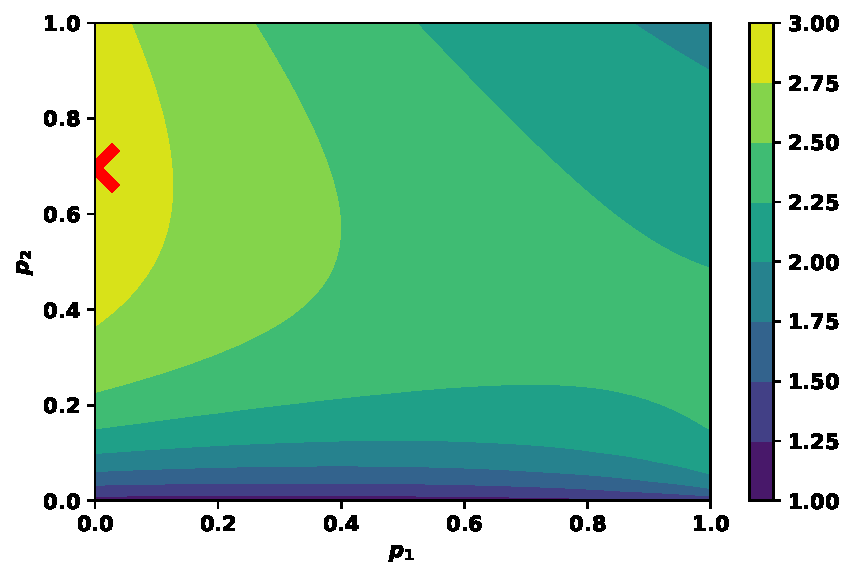
\includegraphics[width=.6\linewidth]{src/chapters/05/reactive_best_response.pdf}
    \caption{The utility of a \(p=(p_1, p_2)\) reactive player against \(q =
    (0.513, 0.773, 0.870, 0.008)\) for changing values of \(p_1\) and \(p_2\).
    The point marked with X is the point identified as the best response.}
    \label{fig:reactive_example_utility}
\end{figure}

Sylvester's formulation can only handle systems of 2 polynomials, however, the
multivariate resultants can be calculated for \(n\) homogeneous polynomials in \(n\)
variables. A number of
multivariate resultants can be found in the literature such as
Dixon's~\cite{ResultantKapur} resultant and Macaulay's~\cite{Macaulay1902}
resultant.

Project~\cite{sympy} which was used to construct Sylvester's resultant is called
SymPy and it is the Pythonic package for symbolic mathematics. However, the
project did not include the feature to calculate multivariate resultants. As
part of this Chapter the source code for constructing both Dixon's and
Macaulay's resultants was developed and was integrated into
SymPy. Figure~\ref{fig:sympy_pr} shows the pull request made to
SymPy for integrating the source code to their codebase.
Figure~\ref{fig:dixon_example} demonstrates an example of using~\cite{sympy} to
calculate Dixon's resultant.

\begin{figure}[!htbp]
    \centering
    
\includegraphics[width=.77\linewidth]{src/chapters/05/pr_screenshot}
    \caption{Screenshot of the pull request made to SymPy for integrating the
    source code of the multivariate resultants to the project's codebase.
    The details of the pull request as well as the conversation with the
    project's main contributors can be found at:~\url{https://github.com/sympy/sympy/pull/14370}.}
    \label{fig:sympy_pr}
\end{figure}

\begin{figure}[H]
\begin{usagepy}
>>> from sympy.polys.multivariate_resultants import DixonResultant
>>> p_1, p_2 = sym.symbols('p_1, p_2')

>>> f = p_1 + p_2
>>> g = p_1 ** 2 + p_2 ** 3
>>> h = p_1 ** 2 + p_2

>>> dixon = DixonResultant(variables=[p_1, p_2], polynomials=[f, g, h])
>>> poly = dixon.get_dixon_polynomial()
>>> matrix = dixon.get_dixon_matrix(polynomial=poly)
>>> matrix
Matrix([
[ 0,  0, -1,  0, -1],
[ 0, -1,  0, -1,  0],
[-1,  0,  1,  0,  0],
[ 0, -1,  0,  0,  1],
[-1,  0,  0,  1,  0]])

>>> matrix.det()
0

\end{usagepy}
\caption{Code example of using~\cite{sympy} to calculate Dixon's resultant.
\(f, g\) and \(h\) have a common root (\(x=1, y=-1\)). The determinant
of Dixon's matrix falls to zero which confirms that the system has a common root.}\label{fig:dixon_example}
\end{figure}

Multivariate resultants theoretically can be used to explicitly identify best
response memory-one strategies by solving the system of 4 polynomials. However,
as previously stated for large systems building the resultant quickly becomes
intractable. As a result in section~\ref{section:numerical_experiments}
a numerical approach was considered instead.

\section{Numerical experiments} \label{section:numerical_experiments}

As briefly discussed in section~\ref{section:introduction}, ZDs have been
praised for their robustness against a single opponent. ZDs are evidence that
extortion works in pairwise interactions. Their behaviour ensures that the
strategies will never lose a game. However, this thesis argues that in multi
opponent interactions, where the payoffs matter, strategies trying to exploit
their opponents will suffer. Compared to ZDs, best response memory-one
strategies which have a theory of mind of their opponents, utilise their
behaviour in order to gain the most from their interactions. The question that
arises then is whether best response strategies are optimal because they behave
in an extortionate way. This is explored in
section~\ref{subsection:best_response_n_2}.

The other main finding presented in~\cite{Press2012} was that short memory of
the strategies was all that was needed. This thesis argues that the second
limitation of ZDs in multi opponent interactions is that of their restricted
memory. To demonstrate the effectiveness of memory in the IPD a best response
longer-memory strategy against a given set of memory-one opponents is explored,
and it's performance is compared to that of a memory-one best response in
section~\ref{subsection:longer_memory_best_response}.

The results of this section rely on estimating best response memory-one
strategies and understanding whether they behave in an extortionate way. Best
responses will be estimated heuristically using Bayesian optimisation, which is
described in section~\ref{section:bayesian_optimisation}, and in order to
investigate whether best responses behave in an extortionate matter the SSE
method described in section~\ref{section:sse} is used.

\subsection{Bayesian optimisation}\label{section:bayesian_optimisation}

Bayesian optimisation is a global optimisation
algorithm that has proven to outperform many other popular
algorithms~\cite{Jones2001}. The algorithm builds a bayesian understanding of
the objective function which is well suited to the potential multiple local optimas in
the described search space of this Chapter. Differential evolution~\cite{Storn1997}
was also considered, however, it was not selected due to Bayesian optimisation being
computationally more efficient.

As described in~\cite{Frazier2018} Bayesian optimisation consists of two main
components: a Bayesian statistical model for modelling the objective function,
and an acquisition function for deciding where to sample next. The algorithm
initially evaluates the objective according to a space-filling experimental
design, often consisting of points chosen uniformly at random. They are used
iteratively to allocate the remainder of a budget of \(I\) function evaluations, as
shown in Algorithm~\ref{algorithm:bayesian_opt}.

\begin{algorithm}[H]
Place a Gaussian process prior on \(f\)\;
Observe \(f\) at \(i_0\) points according to an initial space-filling experimental design, set \(i = i_0\) \;
\While{ \(i \leq I\)}{
Update the posterior probability distribution on \(f\) using all available data\;
Let \(x_i\) be a maximiser of the acquisition function over \(x\), where the acquisition function is computed using the current posterior distribution\;
Observe \(y_i\) = \(f(x_i)\)\;
Increment \(i\)\;
}
\Return either the point evaluated with the largest \(f(x)\), or the point with the largest posterior mean.
\caption{Basic pseudo-code for Bayesian optimisation. As given in~\cite{Frazier2018}}\label{algorithm:bayesian_opt}
\end{algorithm}

The statistical model is invariably a Gaussian process. It provides a Bayesian
posterior probability distribution that describes potential values for the
objective function at a candidate point. Each time the objective function is
observed at the new point the posterior distribution is updated.

The acquisition function measures the value that would be generated by
evaluation of the objective function at a new point, based on the current
posterior distribution over \(f\). The most commonly used acquisition
functions are:

\begin{itemize}
    \item The expected improvement~\cite{Jones1998}.
    \item The knowledge gradient~\cite{Frazier2009}.
    \item The entropy search and predictive entropy search~\cite{Hennig2012}.
\end{itemize}

As an example of the algorithm's usage consider the optimisation problem of
(\ref{eq:mo_tournament_optimisation}). Figure~\ref{bayesian_example} illustrates
the change of the utility function over \(I\). The algorithm is set to run for
\(I=60\). After 60 function evaluations if the utility has not changed in the
last 10\% of evaluations, then the algorithm runs for a further 20 evaluations.
This is repeated until there is no change to the utility in the last 10\% of
evaluations.

\begin{figure}[!htbp]
    \begin{center}
    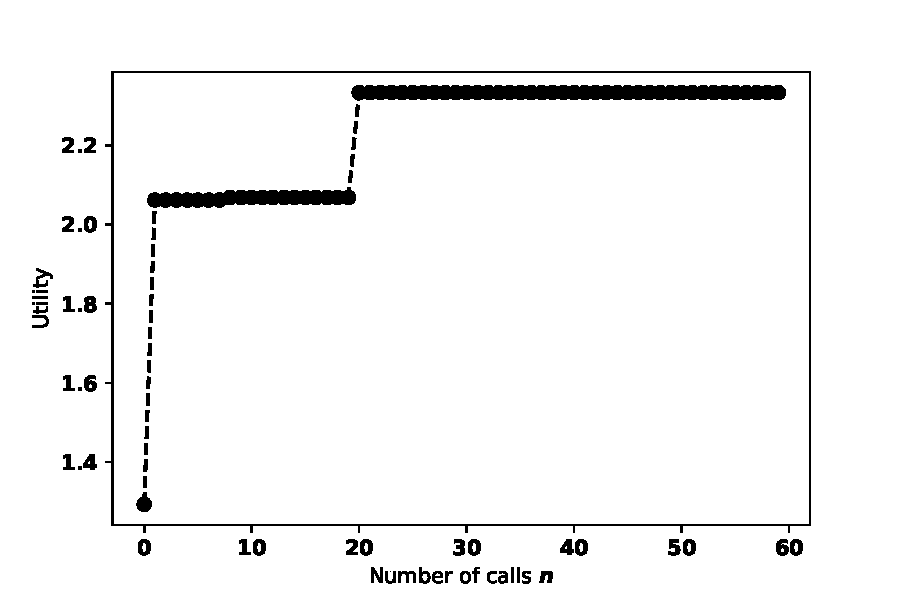
\includegraphics[width=.65\linewidth]{src/chapters/05/paper/memory-size-in-the-prisoners-dilemma/img/bayesian_example.pdf}
    \end{center}
    \caption{Utility over time of calls using Bayesian optimisation. The
    opponents are \(q^{(1)} = (\frac{1}{3}, \frac{1}{3}, \frac{1}{3},
    \frac{1}{3})\) and \(q^{(2)} = (\frac{1}{3}, \frac{1}{3},
    \frac{1}{3}, \frac{1}{3})\). The best response obtained is \(p^* = (0, \frac{11}{50}, 0, 0)\)}
    \label{bayesian_example}
\end{figure}

\subsection{SSE method}\label{section:sse}

The SSE method is a linear algebraic approach that defines the closest ZD
strategy to a given strategy \(p\). This strategy is defined as \(x^*\) given
by,

\begin{equation}\label{eqn:x_star_formula}
    x^* = {\left(C^{T}C\right)}^{-1}C^{T}\bar{p}
\end{equation}

where

\[\bar{p}=(p_1 - 1, p_2 - 1, p_3, p_4) \text{ and}\] and

\begin{equation}\label{eq:definition_of_C}
    C =
    \begin{bmatrix}
        R - P & R- P \\
        S - P & T- P \\
        T - P & S- P \\
        0     & 0 \\
    \end{bmatrix}.
\end{equation}

Once \(x^*\) is estimated the method calculates the squared norm of the
remaining error referred to as sum of squared errors of prediction (SSE):

\begin{equation}\label{eqn:x_SSError_formula}
    \text{SSE} = {\bar{p}} ^ T \bar{p} -
           \bar{p} C \left(C ^ T C \right) ^ {-1} C ^ T \bar{p}
         = {\bar{p}} ^ T \bar{p} - \bar{p} C x ^ *
\end{equation}

The SSE is defined as how far a strategy is from behaving as a ZD. A small SSE
implies ZD behaviour whereas a high SSE implies a non extortionate behaviour.

\subsection{Best response memory-one strategies for \(N=2\)}\label{subsection:best_response_n_2}

Bayesian optimisation was used to generate a data set of best response
memory-one strategies for \(N=2\) opponents. The data set has been archived and
is available at~\cite{glynatsi2019}. The data set contains two sets of best
response memory-one strategies for each pair of opponents. These are:

\begin{itemize}
    \item Best response memory-one strategies without self interactions.
    \item Best response memory-one strategies with self interactions.
\end{itemize}

In several evolutionary settings such as Moran Processes self interactions are
key. Previous work has identified interesting results such as the appearance of
self recognition mechanisms when training strategies using evolutionary
algorithms in Moran processes~\cite{Knight2018}. This aspect of reinforcement
learning can be done for best response memory-one strategies by incorporating
the strategy itself in the objective function as shown in
Equation~(\ref{eq:mo_tournament_optimisation}). \(K\) is the number of self
interactions that will take place.

\begin{equation}\label{eq:mo_evolutionary_optimisation}
    \begin{aligned}
    \max_p: & \ \frac{1}{N} \sum\limits_{i=1} ^ {N} {u_q}^{(i)} (p) + Ku_p(p)
    \\
    \text{such that}: & \ p \in \R_{[0, 1]}
    \end{aligned}
   \end{equation}

For determining the memory-one best response with self interactions, an
algorithmic approach is considered, called \textit{best response dynamics}. The
best response dynamics approach used in this manuscript is given by
Algorithm~\ref{algo:best_response_dynamics}.

\begin{algorithm}[H]
    $p^{(t)}\leftarrow (1, 1, 1, 1)$\;
    \While{$p^{(t)} \neq p ^{(t -1)}$}{
    $p^{(t + 1)} =  \text{argmax} \frac{1}{N} \sum\limits_{i=1} ^ {N} {u_q}^{(i)}
    (p^{(t)}) + Ku_{p^{(t)}}(p^{(t)})$\;
    }
    \caption{Best response dynamics algorithm}
    \label{algo:best_response_dynamics}
 \end{algorithm}

Using this approach it would be possible to create a memory-one best response
strategy that updates on every generation of a Moran process to recalculate the
optimal behaviour given the population.

The data set contains a total of 1,000 trials corresponding to 1,000 different
instances of a best response strategy in tournaments with and without self
interactions. For each trial a set of 2 opponents is randomly generated and the
memory-one best responses against them are found. The probabilities \(q_i\) of
the opponents are randomly generated and
Figures~\ref{fig:first_opponents_probabilities} and
\ref{fig:second_opponents_probabilities}, show that they are uniformly
distributed over the trials. Thus, the full space of possible opponents has been
covered.

\begin{figure}[!htbp]
    \begin{subfigure}{0.5\textwidth}
        \centering
        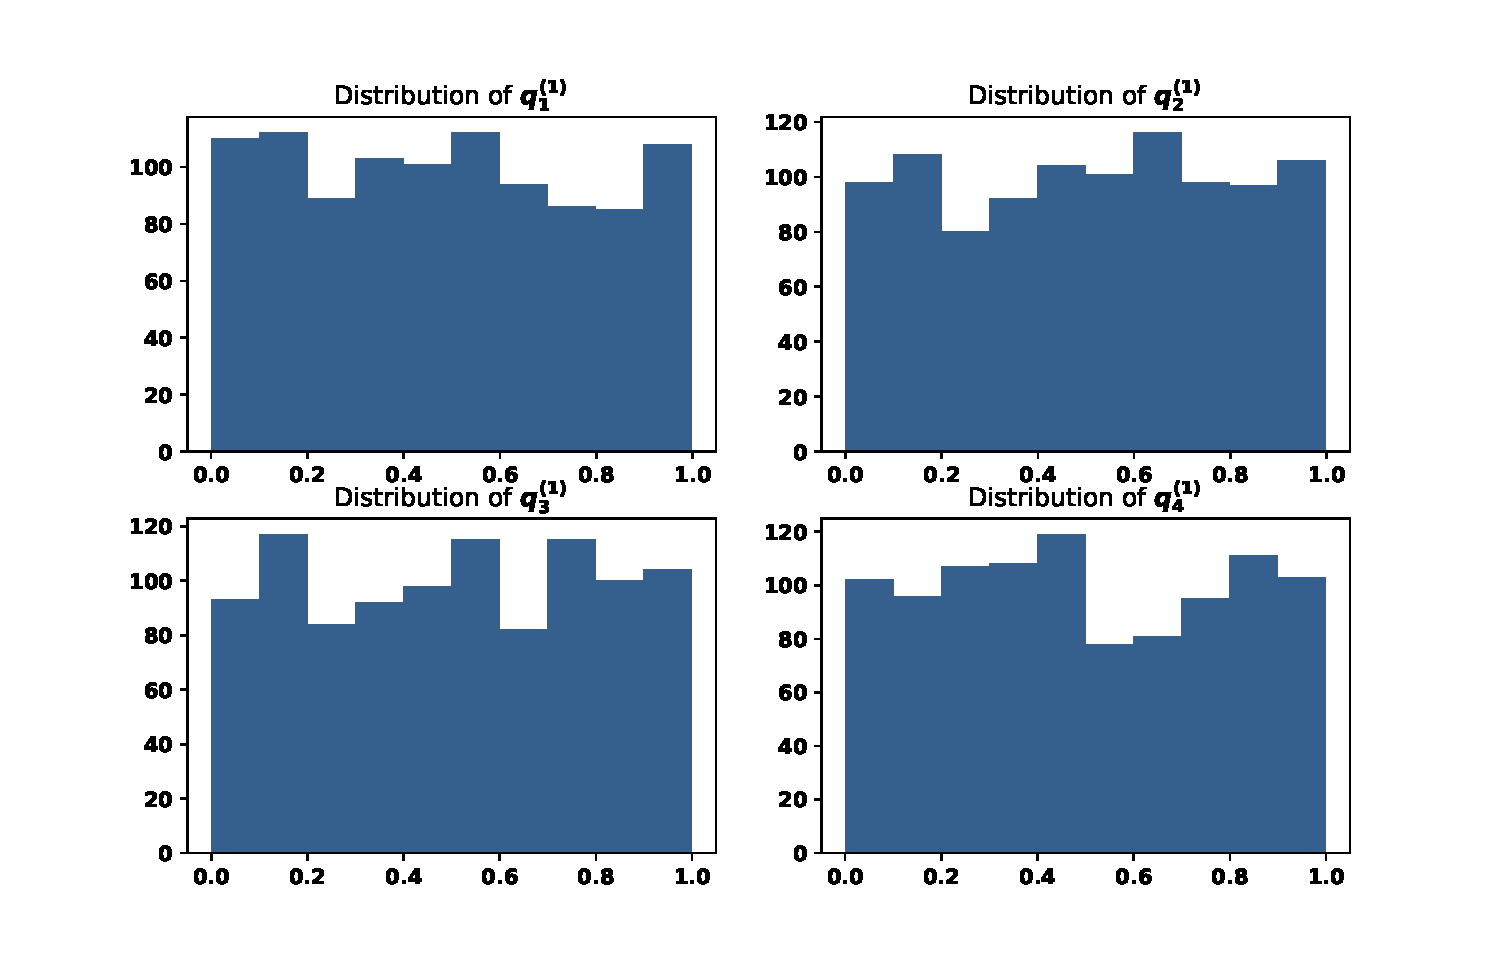
\includegraphics[width=\linewidth]{src/chapters/05/paper/memory-size-in-the-prisoners-dilemma/img/first_opponent_probabilities.pdf}
        \subcaption{Distributions of first opponents' probabilities.}
        \label{fig:first_opponents_probabilities}
    \end{subfigure}
    \begin{subfigure}{0.5\textwidth}
        \centering
        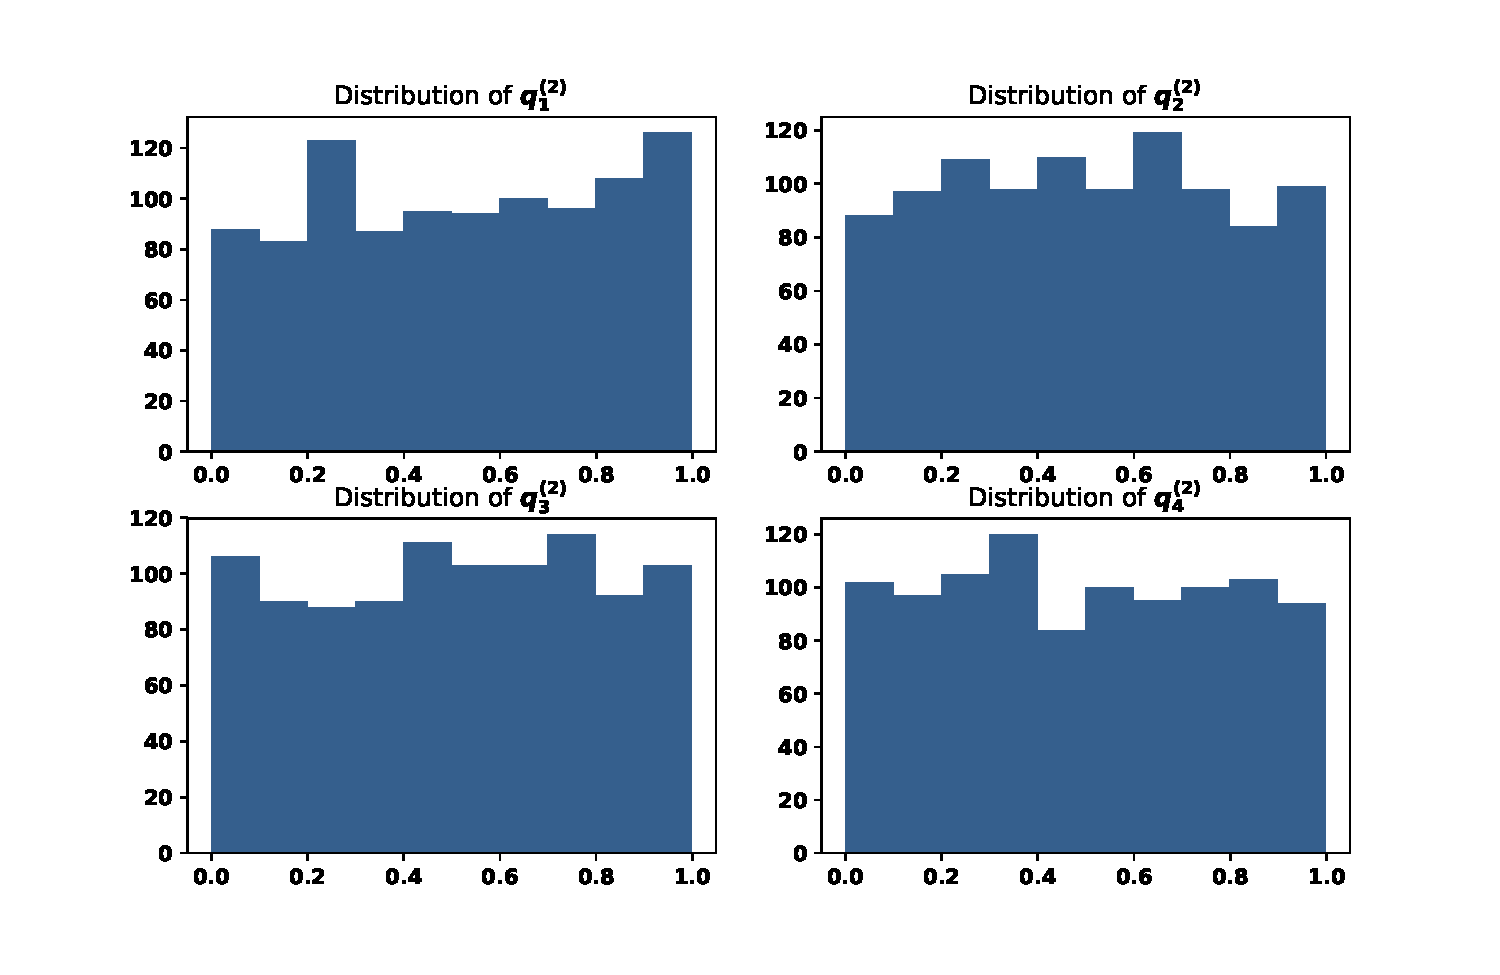
\includegraphics[width=\linewidth]{src/chapters/05/paper/memory-size-in-the-prisoners-dilemma/img/second_opponent_probabilities.pdf}
        \subcaption{Distributions of second opponents' probabilities.}
        \label{fig:second_opponents_probabilities}
    \end{subfigure}
    \caption{Distributions of opponents' probabilities.}
\end{figure}

The SSE method was applied to the best response memory-one strategies once the
data set was generated. The distributions of SSE for the best response in
tournaments \((N = 2)\) with and without self interactions with \((K = 1)\) are
given in Figure~\ref{fig:sse_distributions}. Moreover, a statistical summary of
the SSE distributions is given in Table~\ref{table:sserror_stats}.

\begin{table}[!htbp]
    \begin{center}
    \resizebox{\columnwidth}{!}{%
    \begin{tabular}{lrrrrrrrrrrr}
        \toprule
        & mean & standard deviation  & 5\% & 50\% &  95\% & max & median & skewness & kurtosis \\
        \midrule
    \textbf{Tournament without self interactions} & 0.34  & 0.40  & 0.028  & 0.17  &
    1.05  & 2.47  & 0.17  & 1.87 & 3.60 \\
    \textbf{Tournament with self interactions} & 0.17 & 0.23 & 0.01 &
    0.12 & 0.67 & 1.53 & 0.12 & 3.42 & 1.92 \\
        \bottomrule
    \end{tabular}}
    \end{center}
    \caption{SSE of best response memory-one for \(N=2\).}\label{table:sserror_stats}
\end{table}

\begin{figure}[!htbp]
    \begin{subfigure}{0.5\textwidth}
        \begin{center}
            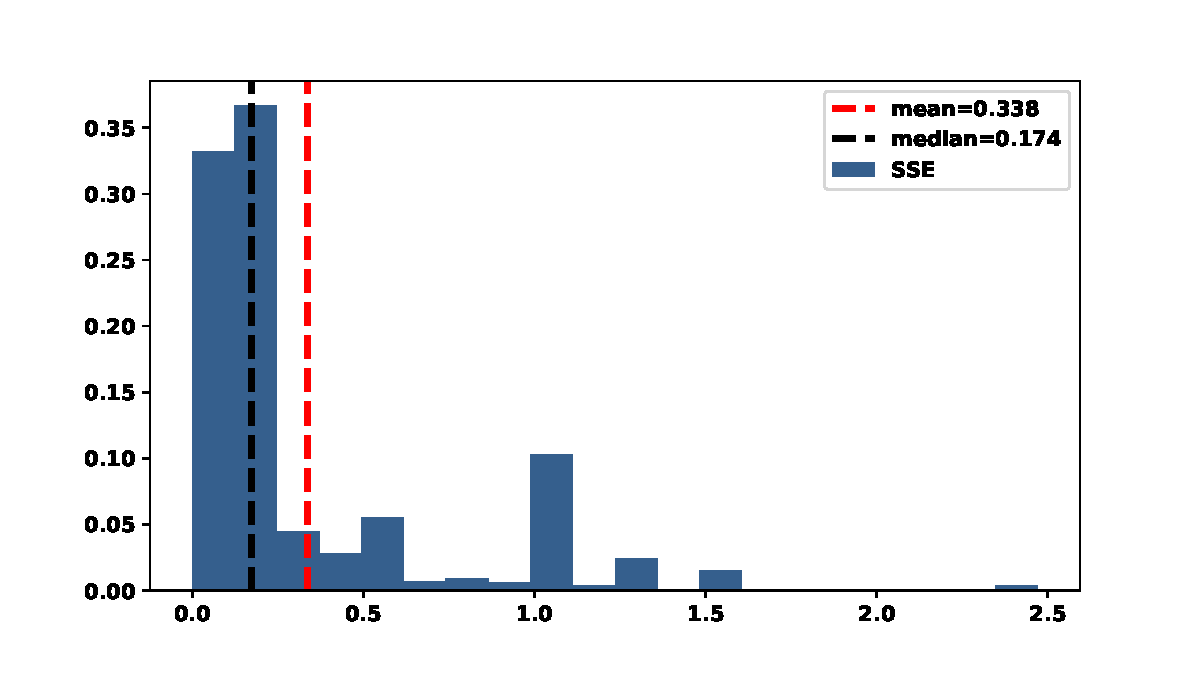
\includegraphics[width=\linewidth]{src/chapters/05/paper/memory-size-in-the-prisoners-dilemma/img/best_respones_sserror.pdf}
        \end{center}
        \caption{SEE distribution for best response in tournaments without self interactions.}
    \end{subfigure}\hfill
    \begin{subfigure}{0.5\textwidth}
        \begin{center}
            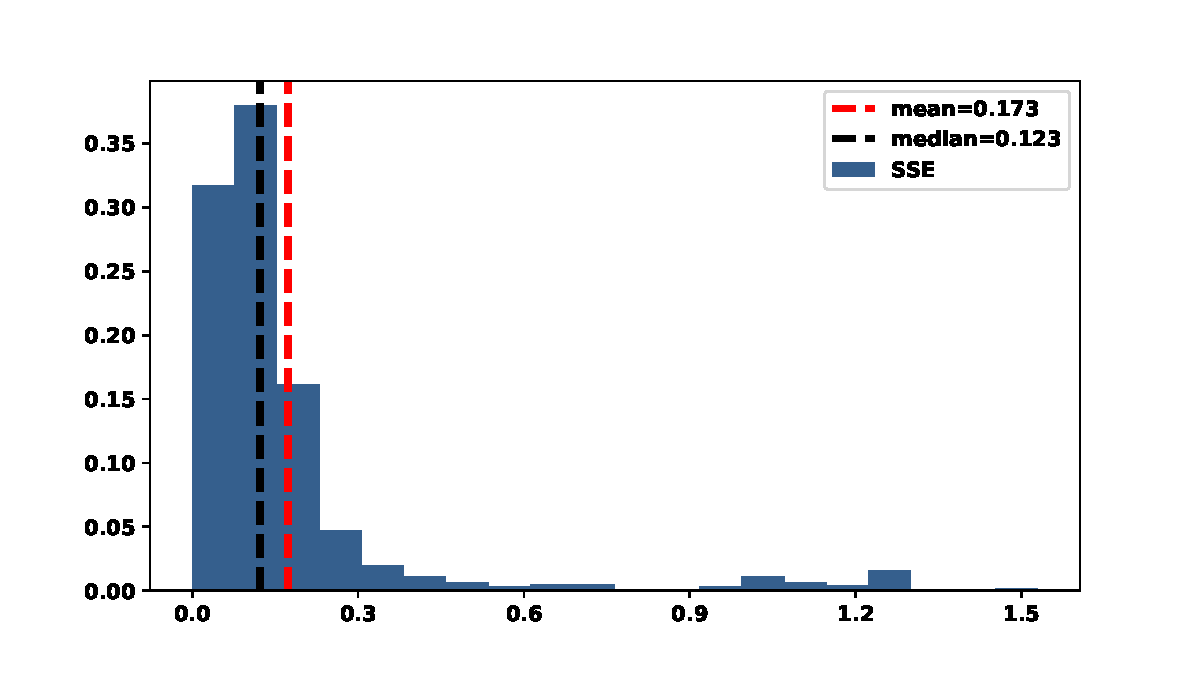
\includegraphics[width=\linewidth]{src/chapters/05/paper/memory-size-in-the-prisoners-dilemma/img/evo_sserror.pdf}
        \end{center}
        \caption{SEE distribution for best response in tournaments with self interactions.}
    \end{subfigure}
    \caption{SEE distributions for best response in tournaments without and with self interactions for \(N=2\).}\label{fig:sse_distributions}
\end{figure}

For the best response in tournaments that do not include self interactions the
distribution of SSE is skewed to the left, indicating that the best response
does exhibit ZDs behaviour and so could be extortionate, however, the best
response is not uniformly a ZDs. A positive measure of skewness and kurtosis,
and a mean of 0.34 indicate a heavy tail to the right. Therefore, in several
cases the strategy is not trying to extort its opponents. In~\cite{Hilbe2018} a
similar behaviour is refereed to as the \textit{partner strategy}. The partner
strategy aims to share the payoff for mutual cooperation, but it is ready to
fight back when being exploited. The partner strategy was designed, but the best
responses which are defined by their opponents seem to exhibit the same
behaviour.

Similarly, when considering self interactions, the distribution of SSE for the
best response strategy has skewness and kurtosis that indicate a heavy tail to
the right. This indicates that memory-one strategies that interact with copies
of themselves need to even
more adaptable than ZDs, and aim for mutual cooperation as well as
exploitation which is in line with the results of \cite{Hilbe2018} where their
strategy was designed to adapt and was shown to be evolutionary stable. The
findings of this work show that an optimal strategy acts in the same way.

The difference between best responses in tournaments without and with self
interactions is further explored by Figure~\ref{fig:behaviour_violin_plots}.
Though, no statistically significant differences have been found, from
Figure~\ref{fig:behaviour_violin_plots}, it seems that the best response that
incorporate self interactions has a higher median $p_2$; which corresponds to
the probability of cooperating after receiving a defection. Thus, they are more
likely to forgive after being tricked. This is due to the fact that they could
be playing against themselves, and they need to be able to forgive so that
future cooperation can occur.

\begin{figure}[!htbp]
    \centering
    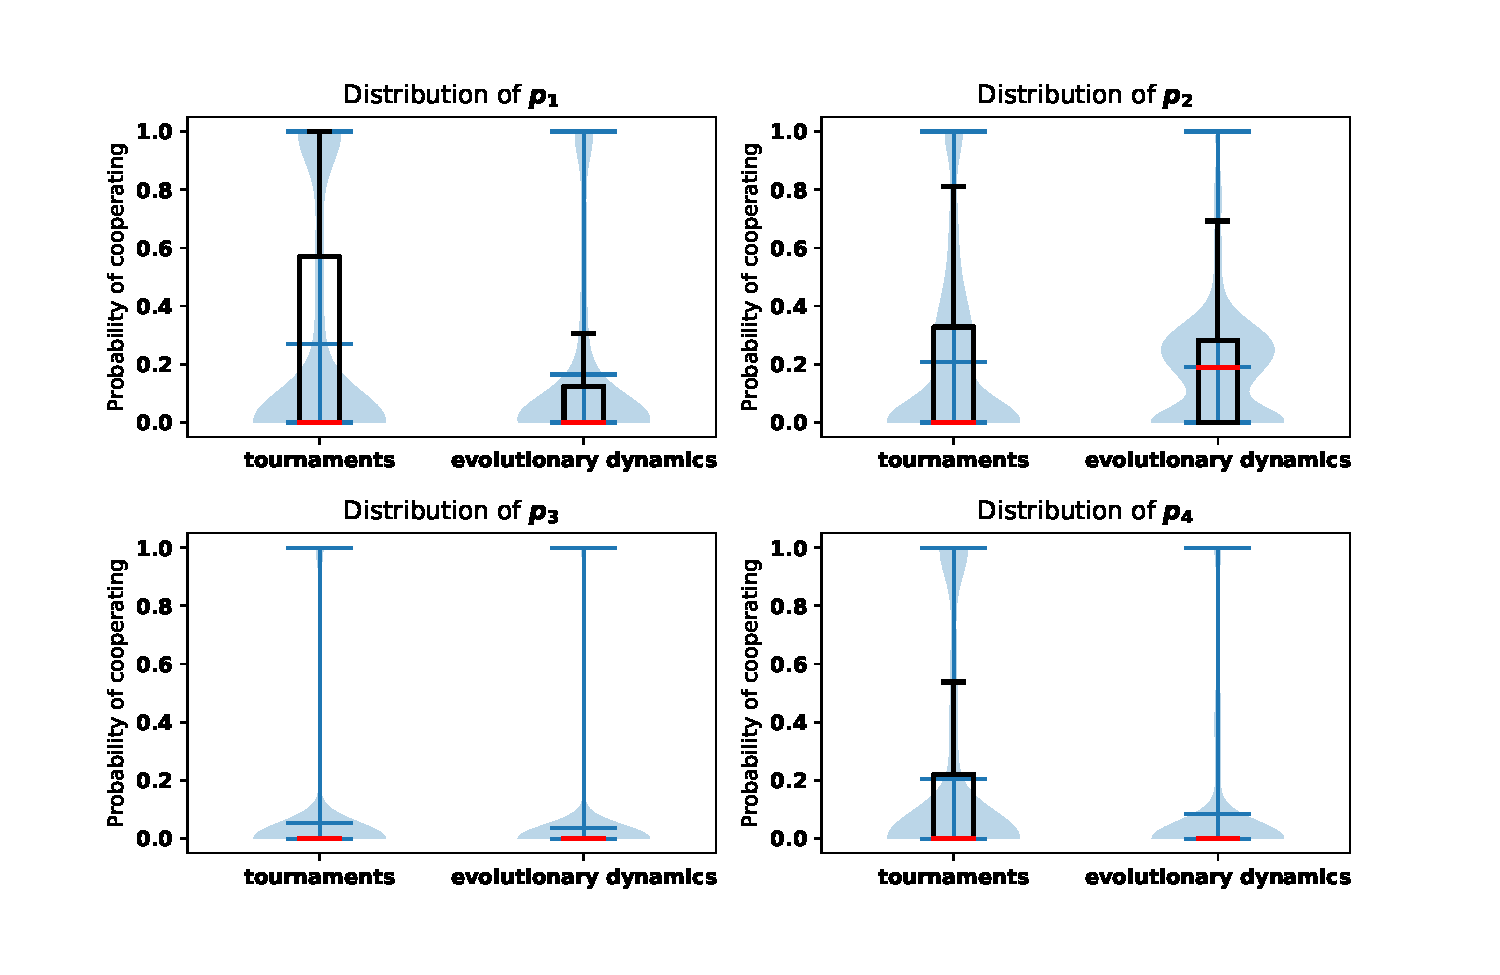
\includegraphics[width=.9\textwidth]{src/chapters/05/paper/memory-size-in-the-prisoners-dilemma/img/behaviour_violin_plots.pdf}
    \caption{Distributions of \(p^*\) for best response in tournaments without
     and with self interactions. The medians, denoted as \(\bar{p}^*\), for
     tournaments are \(\bar{p}^* = (0, 0, 0, 0)\), and for evolutionary settings
     \(\bar{p}^* = (0, 0.19, 0, 0)\).}
    \label{fig:behaviour_violin_plots}
\end{figure}

\subsection{Longer memory best responses}\label{subsection:longer_memory_best_response}

This section focuses on the memory size of strategies. The effectiveness of
memory in the IPD has been previously explored in the literature, as
discussed in section~\ref{section:introduction}, however, none of the
previous works has compared the performance of longer-memory strategies to
memory-one best responses.

The strategy used in this Chapter is one of the archetypes described in Chapter
\ref{chapter:literature_review} called Gambler (introduced
in~\cite{Harper2017}). As a reminder, Gambler is a stochastic version of a lookup
table. It makes probabilistic decisions based on the opponent's \(n_1\) first
moves, the opponent's \(m_1\) last moves and the player's \(m_2\) last moves.
In this Chapter Gambler with parameters: $n_1 = 2, m_1 = 1$ and $m_2
= 1$ is used as a longer-memory strategy.

By considering the opponent's first two moves, the opponents last move and the
player's last move, there are only 16 $(4 \times 2 \times 2)$ possible outcomes
that can occur, furthermore, Gambler also makes a probabilistic decision of
cooperating in the opening move. Thus, Gambler is a function \(f: \{\text{C,
D}\} \rightarrow [0, 1]_{\R}\). This can be hard coded as an element
of \([0, 1]_{\R} ^ {16 + 1}\), one probability for each outcome plus the opening
move. Hence, compared to (\ref{eq:mo_tournament_optimisation}), finding an
optimal Gambler is a 17 dimensional problem given by:

\begin{equation}\label{eq:gambler_optimisation}
    \begin{aligned}
    \max_p: & \ \sum_{i=1} ^ {N} {U_q}^{(i)} (f)
    \\
    \text{such that}: & \ f \in \R_{[0, 1]}^{17}
    \end{aligned}
\end{equation}

Note that Equation~(\ref{eq:tournament_utility}) can not be used here for the
utility of Gambler, and actual simulated players are used. This is done using a
tournament of 500 turns and 200 repetitions, moreover,
(\ref{eq:gambler_optimisation}) is solved numerically using Bayesian
optimisation.

Similarly to the previous section, a large data set has been generated with
instances of an optimal Gambler and a memory-one best response, available
at~\cite{glynatsi2019}. Estimating a best response Gambler (17 dimensions) is
computational more expensive compared to a best response memory-one (4
dimensions). As a result, the analysis of this section is based on a total of
130 trials. For each trial two random opponents have been selected. The 130 pair
of opponents are a sub set of the opponents used in
section~\ref{subsection:best_response_n_2}. The distributions of their
transition probabilities are given in Figures
\ref{fig:first_opponents_probabilities_with_gambler} and
\ref{fig:first_opponents_probabilities_with_gambler}.

\begin{figure}[!htbp]
    \begin{subfigure}{0.5\textwidth}
        \centering
        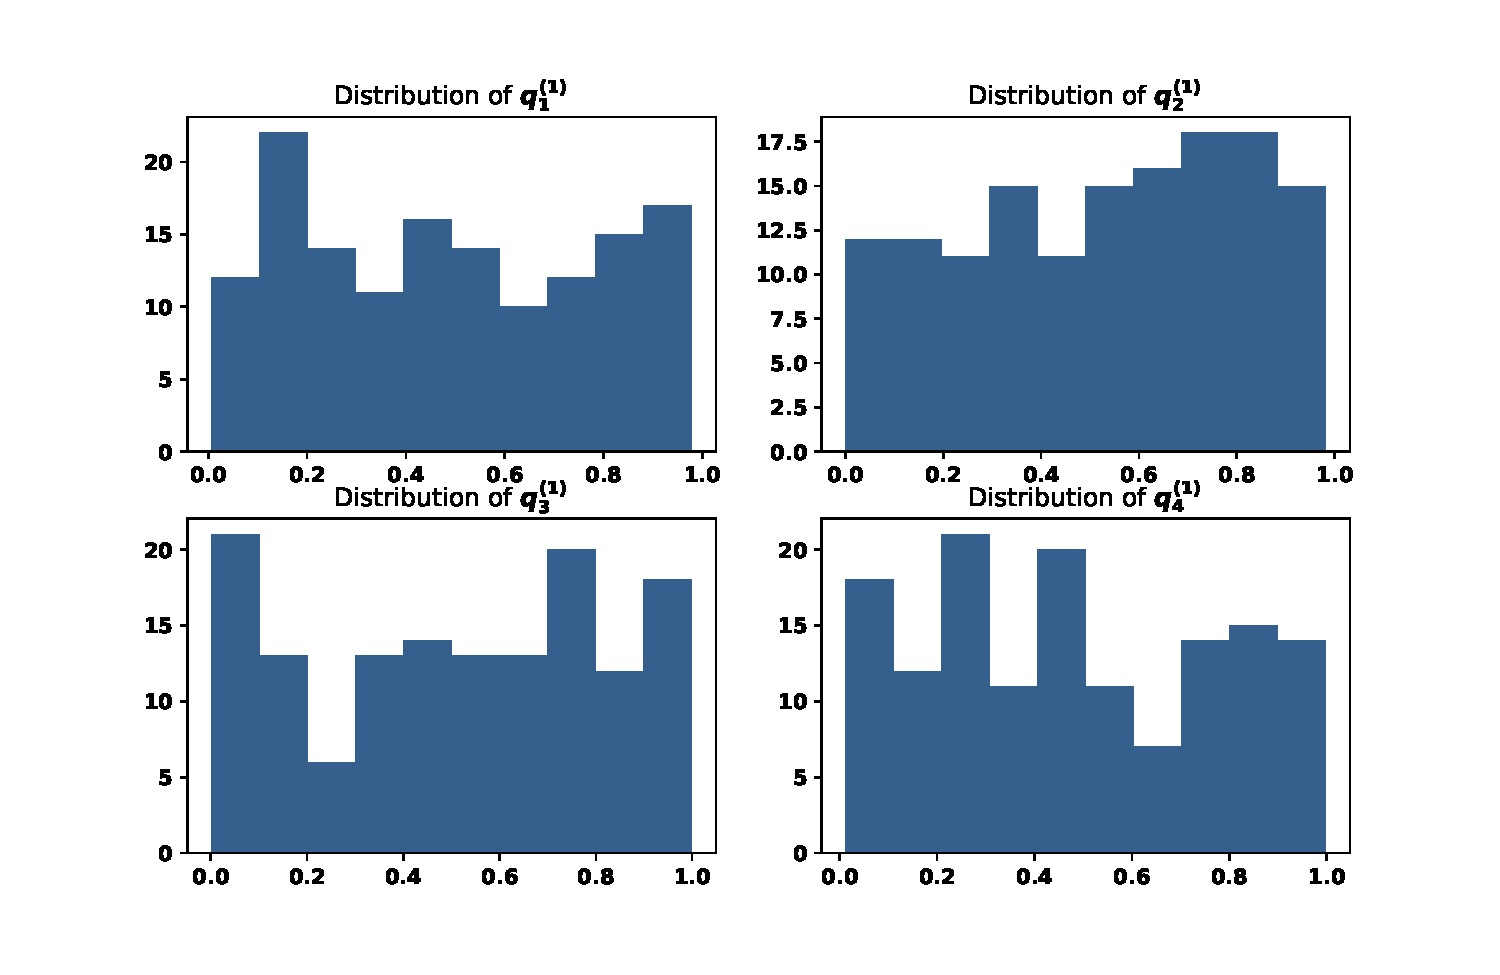
\includegraphics[width=\linewidth]{src/chapters/05/paper/memory-size-in-the-prisoners-dilemma/img/first_opponent_probabilities_with_gambler.pdf}
        \subcaption{Distributions of first opponents' probabilities for longer memory experiment.}
        \label{fig:first_opponents_probabilities_with_gambler}
    \end{subfigure}
    \begin{subfigure}{0.5\textwidth}
        \centering
        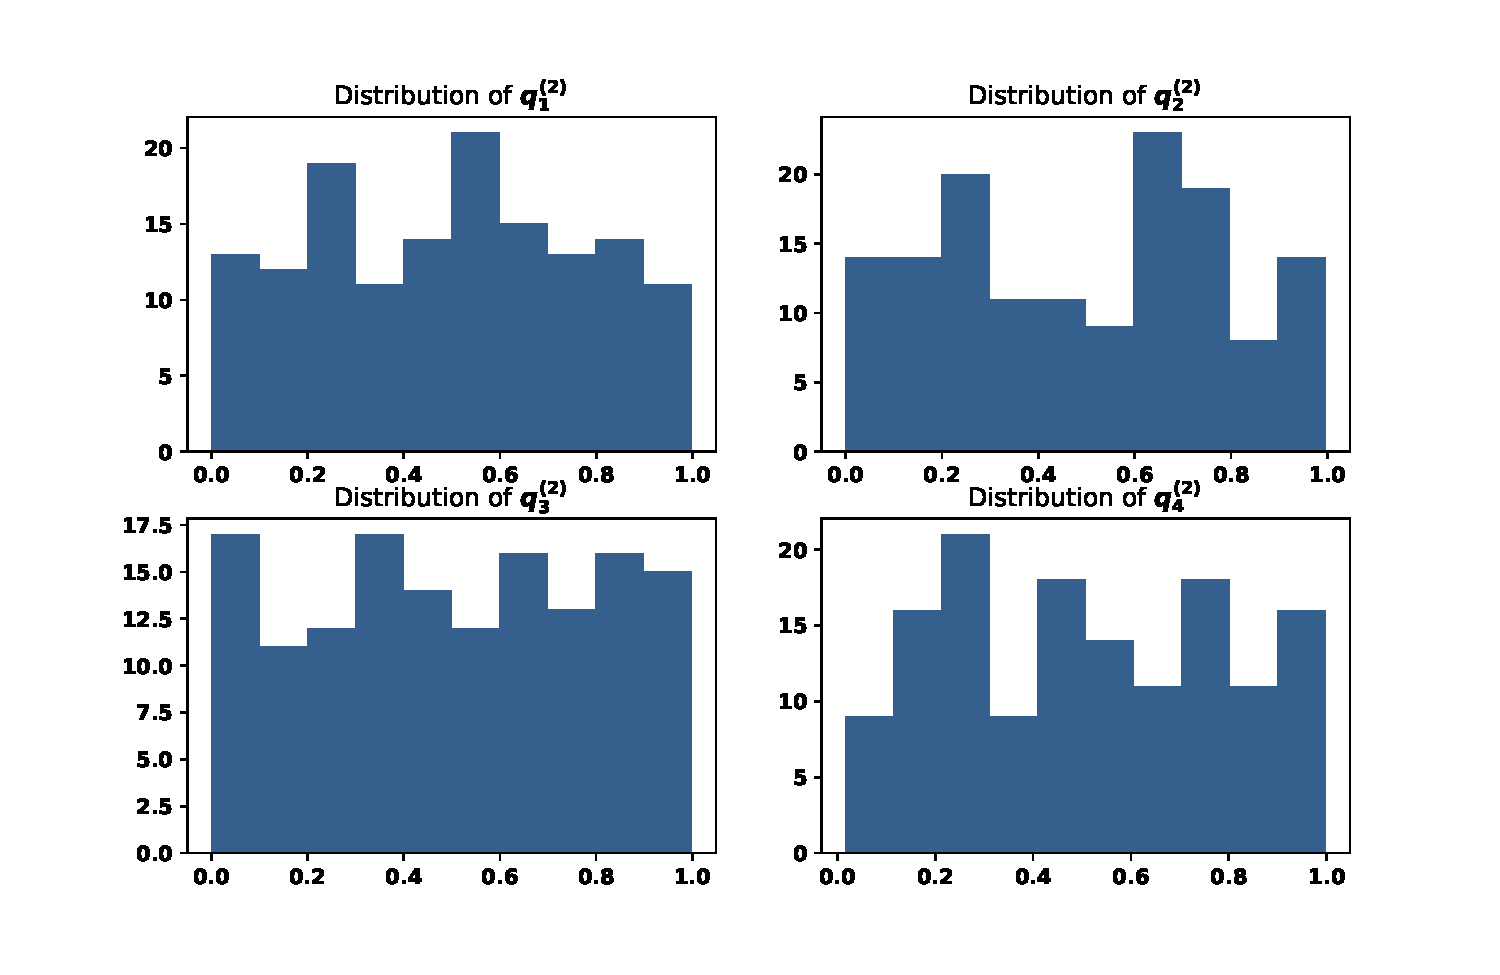
\includegraphics[width=\linewidth]{src/chapters/05/paper/memory-size-in-the-prisoners-dilemma/img/second_opponent_probabilities_with_gambler.pdf}
        \subcaption{Distributions of second opponents' probabilities for longer memory experiment.}
        \label{fig:second_opponents_probabilities_with_gambler}
    \end{subfigure}
    \caption{Distributions of opponents' probabilities for longer memory experiment.}
\end{figure}

The ratio between Gambler's utility and the best response memory-one strategy's utility has been calculated and its distribution in
given in Figure~\ref{fig:utilities_gambler_mem_one}.
It is evident from Figure~\ref{fig:utilities_gambler_mem_one} that
Gambler always performs as well as the best response memory-one strategy and often performs better. There are
no points where the ratio value is less than 1, thus Gambler never performed less
than the best response memory-one strategy and in places outperforms it. This seems to be at odd with the
result of~\cite{Press2012} that against a memory-one opponent having a longer memory
will not give a strategy any
advantage. However, against two memory-one opponents Gambler's performance is better than
the optimal memory-one strategy. This is evidence that in the case of two opponents having a
shorter memory is limiting.

\begin{figure}[!htbp]
    \centering
    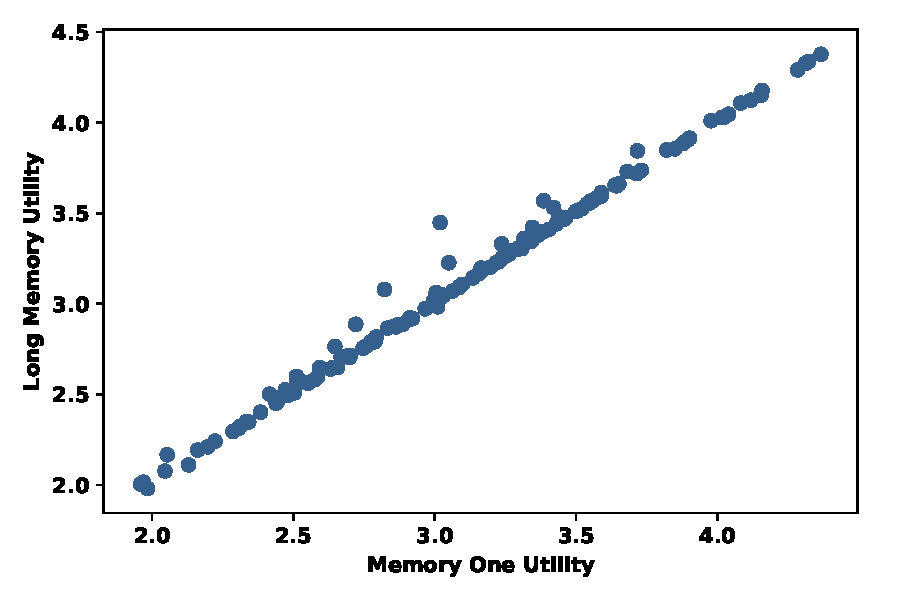
\includegraphics[width=.65\textwidth]{src/chapters/05/paper/memory-size-in-the-prisoners-dilemma/img/gambler_performance_against_mem_one.pdf}
    \caption{Utilities of Gambler and best response memory-one strategies for
    130 different pair of opponents.}\label{fig:utilities_gambler_mem_one}
\end{figure}

\section{Stability of defection}\label{section:stability_of_defection}

An additional theoretical result that is possible to obtain due to
Theorem~\ref{theorem:tournament_utility}, is a condition for which in an
environment of memory-one opponents defection is the stable choice, based only
on the coefficients of the opponents.

This result is obtained by evaluating the sign of Equation
(\ref{eq:tournament_utility})'s derivative at \(p=(0, 0, 0, 0)\). If at that
point the derivative is negative, then the utility of a player only decreases if
they were to change their behaviour, and thus defection at that point is stable.

\begin{lemma}\label{lemma:stability_of_defection}
    In a tournament of \(N\) players \(\{q^{(1)}, q^{(2)}, \dots, q^{(N)} \}\)
    for \(q^{(i)} \in \R_{[0, 1]} ^ 4\)
    defection is stable if the transition probabilities of the
    opponents satisfy conditions Equation~(\ref{eq:defection_condition_one}) and Equation~(\ref{eq:defection_condition_two}).

    \begin{equation}\label{eq:defection_condition_one}
        \sum_{i=1} ^ N (c^{(i)T} \bar{a}^{(i)} - \bar{c}^{(i)T} a^{(i)}) \leq 0
    \end{equation}

    while,

    \begin{equation}\label{eq:defection_condition_two}
        \sum_{i=1} ^ N \bar{a}^{(i)} \neq 0
    \end{equation}
\end{lemma}

\begin{proof}
    For defection to be stable the derivative of the utility
    at the point \(p = (0, 0, 0, 0)\) must be negative.

    Substituting \(p = (0, 0, 0, 0)\) in
    Equation (\ref{eq:mo_tournament_derivative}) gives:

    \begin{equation}
        \left.\frac{d\sum\limits_{i=1} ^ {N} {u_q}^{(i)} (p)}{dp} \right\rvert_{p=(0,0,0,0)} =
    \sum_{i=1} ^ N \frac{(c^{(i)T} \bar{a}^{(i)} - \bar{c}^{(i)T} a^{(i)})}
    {(\bar{a}^{(i)})^2}
    \end{equation}

    The sign of the numerator \( \displaystyle\sum_{i=1} ^ N (c^{(i)T} \bar{a}^{(i)} - \bar{c}^{(i)T} a^{(i)})\)
    can vary based on the transition probabilities of the opponents.
    The denominator can not be negative, and otherwise is always positive.
    Thus the sign of the derivative is negative if and only if
    \( \displaystyle\sum_{i=1} ^ N (c^{(i)T} \bar{a}^{(i)} - \bar{c}^{(i)T} a^{(i)}) \leq 0\).
\end{proof}

Consider a population for which defection is known to be stable. In that
population all the members will over time adopt the same behaviour; thus in such
population cooperation will never take over. This is demonstrated in
Figure~\ref{fig:stability_of_defection}.

\begin{figure}[!htbp]
    \centering
    \includegraphics[width=.5\linewidth]{src/chapters/05/paper/memory-size-in-the-prisoners-dilemma/img/stability_of_defection_plots.pdf}
    \caption{A. For \(q_{1}=(0.2219, 0.8707, 0.2067, 0.9186)\),
    $q_{2}=(0.4884, 0.6117, 0.7659, 0.5184)$ and
    $q_{3}=(0.2968, 0.1877, 0.0807, 0.7384)$, Equation~(\ref{eq:defection_condition_one}) and
    Equation~(\ref{eq:defection_condition_two}) hold and \Defector takes over the
    population. \protect\linebreak
    B. For $q_{1}=(0.9670, 0.5472, 0.9726, 0.7148)$,
    $q_{2}=(0.6977, 0.2160, 0.9762, 0.0062)$ and
    $q_{3}=(0.2529, 0.4349, 0.7738, 0.1976)$, Equation~(\ref{eq:defection_condition_one}) fails
    and \Defector does not take over the population.}\label{fig:stability_of_defection}
\end{figure}

\section{Chapter summary}

This Chapter has considered best response strategies in the IPD
game, and more specifically, memory-one best responses. It has proven that:

\begin{itemize}
    \item The utility of a memory-one strategy against a set
          of memory-one opponents can be written as a sum of ratios of quadratic
          forms (Theorem~\ref{theorem:tournament_utility}).
    \item There is a compact way of identifying a memory-one best response to a
        group of opponents through a search over a discrete set
        (Theorem~\ref{theorem:memone_group_best_response}).
    \item There is a compact way of identifying environment of memory-one
    opponents where defection is the stable choice based only on the
    coefficients of the opponents (Lemma~\ref{lemma:stability_of_defection}).
\end{itemize}

Note that Theorem~\ref{theorem:memone_group_best_response} does not only
have game theoretic novelty, but also mathematical novelty of solving quadratic
ratio optimisation problems where the quadratics are non concave. Additionally,
Theorem~\ref{theorem:memone_group_best_response} led to
Lemma~\ref{lemma:reactive_best_response} which defined best response reactive
strategies. Using the set of reactive strategies it was possible to demonstrate
the usage of resultant theory in the search of best response strategies.

The empirical results of this Chapter were presented in
section~\ref{section:numerical_experiments}. The results relied on a bespoke
data set of 1,000 pairs of memory-one opponents. For each pair of opponents two
sets of best response memory-one strategies were estimated. Best responses that
included and not self interactions. The behaviour of these best responses was
investigated. More specifically, it was explored whether it was extortionate
acts that made them the most favourable strategies. It was shown that it was not
extortion but adaptability that allowed the strategies to gain the most from
their interactions. In settings with self interactions there is some evidence
that the best response strategy is more likely to forgive after being tricked.

Section~\ref{section:numerical_experiments} also explored the limitations of
memory. The performance of best response memory-one strategy was compared to
that of a Gambler with longer memory. The results concluded that the
performance of memory-one strategies is limited by their memory in cases where
they interact with multiple opponents. They can never score higher than a
longer memory strategy.

By specifically exploring the entire space of memory-one strategies to identify
the best strategy for a variety of situations, this Chapter has added to the
literature casting doubt on the effectiveness of ZDs, it has highlighted the
importance of adaptability and provides a framework for the continued
understanding of these important questions.
